\allowdisplaybreaks
\chapter{Supplementary Material of Chapter \ref{chap:pinn-bo}} 
\label{section:pinn-bo_supp}
\section{Additional Experimental Details}
\label{section:pinn-bo_experiments_synthetic}
We present the mathematical expressions of five synthetic objective functions and their accompanied PDEs used in Section \ref{section:pinn-bo_experiments} of Chapter \ref{chap:pinn-bo} as follows: 
\paragraph{Drop-Wave:} 
\begin{align*}
    f(\mathbf{x}) &= - \frac{1 + \cos(12\sqrt{\mathbf{x}_1^2 + \mathbf{x}_2^2})}{0.5(\mathbf{x}_1^2 + \mathbf{x}_1^2) + 2} \text{ s.t. } \mathbf{x}_1 \frac{\partial f}{\partial \mathbf{x}_2} - \mathbf{x}_2 \frac{\partial f}{\partial \mathbf{x}_1} = 0
\end{align*}
\paragraph{Styblinski-Tang:}
\begin{align*}
        f(\mathbf{x}) &= \frac{1}{2} \sum_{i=1}^{d} (\mathbf{x}_i^4 - 16\mathbf{x}_i^2 + 5\mathbf{x}_i) \text{ s.t. }  \sum_{i=1}^d \frac{\partial f}{\partial \mathbf{x}_i} = \sum_{i=1}^{d}(2\mathbf{x}_i^3 -16\mathbf{x}_i +\frac{5}{2})
\end{align*}

\paragraph{Rastrigin:}
\begin{align*}
        f(\mathbf{x}) &= 10d + \sum_{i=1}^{d} \left[ \mathbf{x}_i^2 - 10 \cos(2\pi \mathbf{x}_i) \right] 
        \\
        \text{s.t. }  &\mathbf{x}^\top \nabla f(\mathbf{x})  - f(\mathbf{x}) = 10\sum_{i=1}^d \left[ (\cos(2\pi \mathbf{x}_i)) + \pi \mathbf{x}_i (\sin(2\pi \mathbf{x}_i)) - 1 \right]
\end{align*}
\paragraph{Michalewics:}
\begin{align*}
        f(\mathbf{x}) &= -\sum_{i=1}^{d} \sin(\mathbf{x}_i) \sin^{2m}\left(\frac{i\mathbf{x}_i^2}{\pi}\right) \text{ s.t. } \mathbf{h}^\top \nabla f(\mathbf{x}) - f(\mathbf{x}) = 0,\\ & \text{where } \mathbf{h} = [\mathbf{h}_1, \mathbf{h}_2, \dots, \mathbf{h}_d]^\top, \mathbf{h}_i = \left[\frac{\cos(\mathbf{x}_i)}{\sin(\mathbf{x}_i)} + \frac{2\mathbf{x}_i (2m-1)}{\tan(\frac{i\mathbf{x}_i^2}{\pi})}\right]^{-1}
\end{align*}
\paragraph{Cosine Mixture:}
\begin{align*}
    0.1 \sum_{i=1}^d \cos(5\pi\mathbf{x}_i) + \sum_{i=1}^d \mathbf{x}_i^2 \text{ s.t } \sum_{i=1}^d \left(\frac{\partial f}{\partial \mathbf{x}_i} - 2\mathbf{x}_i + 0.5\pi\sin(5\pi\mathbf{x}_i) \right)^2 = 0
\end{align*}

% \subsection{Real-world Applications}
% \label{section:pinn-bo_experiments_real_world}
% \subsubsection{Optimizing Steady-State Temperature}
% \label{section:pinn-bo_experiments_2d_laplace}
% In this study, we showcase the benchmark optimization outcomes achieved by our proposed PINN-BO algorithm, comparing them with baseline methods for the steady-state temperature optimization task.  The governing PDE dictating the temperature distribution is expressed as: $\nabla^2 T(x, y) = 0$. We explore the heat equation in a domain where $x$ and $y$ lie within the defined range of $[0,2\pi]$. To thoroughly investigate the problem, we consider three distinct boundary conditions for this equation, each contributing to a nuanced understanding of the system: 

%  \paragraph{Heat Equation with boundary conditions 1}
%  \label{para:heat1}
%  \begin{align*}
%      T(x, 0) &= 5\sin(y) + \sqrt{1+y} \\
%     T(x, 2\pi) &= y\sin\left(3\cos(y) + 2\exp(y)\sin(y)\right) \\
%    T(0, y) &= 10\cos(x) + x\exp(\sqrt{x^2 + \sin(x)}) \\
%    T(2\pi, y) &= 3\sqrt{\exp(x\exp(-x))}\sin(x) + \cos(3x)\cos(3x)
%  \end{align*}
%  \paragraph{Heat Equation with boundary conditions 2}
%  \label{para:heat2}
% \begin{align*}
%     T(x, 0) &= \sin(x) \cos(2x) + x^2\sqrt{3x}  + e^{\sin(x)} \\
%     T(x, 2\pi) &= e^{\sin(x)} \sqrt{3x} + x^2 \cos(x)  \sin^2(x)   + e^{\cos(x)} \\
%     T(0, y) &= \sqrt{2y}  \sin(y) + y^3\cos(2y)   + e^{\cos(y)} \\
%     T(2\pi, y) &= \sin(y) \cos(2y) + y^3\sqrt{2y}   + e^{\sin(y)}
% \end{align*}
% \paragraph{Heat Equation with boundary conditions 3}
% \label{para:heat3}
% \begin{align*}
%     T(x, 0) &= \left(\sin(x) + \cos(2x) \right) \sqrt{3x} + x^2 + e^{\sin(x)} \\
%     T(x, 2\pi) &= \left(e^{\sin(x)} + \sqrt{3x} \right) \cos(x) + \left(\sin^2(x) + x^2\right)  e^{\cos(x)}
%     \\
%     T(0, y) &= \left(\sqrt{2y} + \sin(y)\right)  \left(\cos(2y) + y^3 \right) + e^{\cos(y)}\\
%     T(2\pi, y) &= \left(\sin(y) + \cos(2y)\right) \left(\sqrt{2y} + y^3\right) + e^{\sin(y)}
% \end{align*}
% We utilized py-pde, a Python package designed for solving partial differential equations (PDEs), available at the following GitHub repository: \url{https://github.com/zwicker-group/py-pde}. This tool enabled us to obtain solutions to heat equations at various input points, with specific boundary conditions serving as the input data. In Figure \ref{fig:heat_dist}, the temperature distribution within the defined domain $[0, 2\pi]$ is visualized. It is important to emphasize that the boundary conditions used for benchmarking purposes are unknown to the methods employed. Adhering to the framework of black-box optimization, we assume that solving the PDEs incurs a substantial computational cost. The figure illustrates the spatial distribution of temperature values $T(x,y)$ across domain $[0, 2\pi] \times [0, 2\pi]$, with each subfigure corresponding to one of the aforementioned boundary conditions. 
% \begin{figure}[ht]
%     \centering
%     \begin{subfigure}[b]{0.3\textwidth}
%         \centering
%         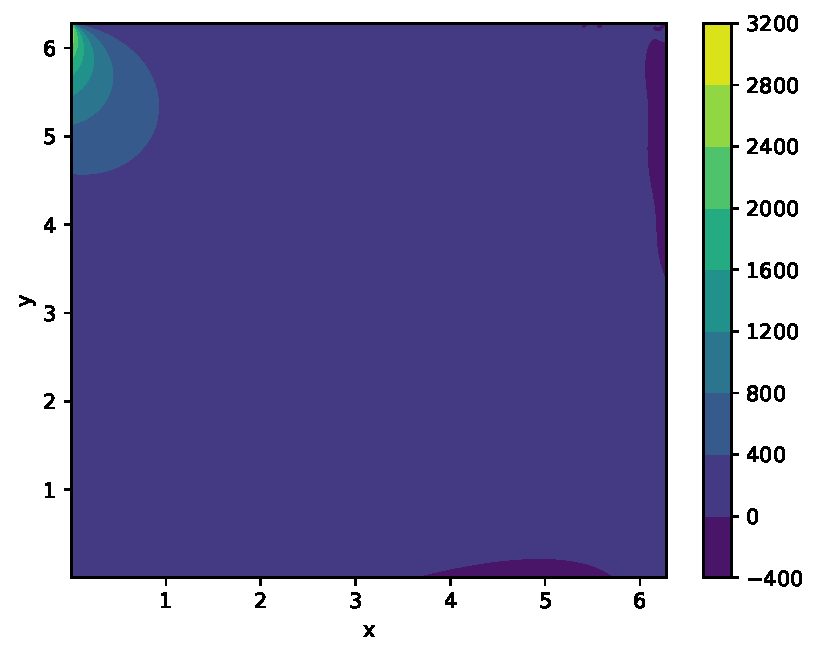
\includegraphics[width=\textwidth]{Figures/PINN-BO/heat_py_pde_1000_test_1.pdf}
%         \caption{Solution of Temperature Equation with boundary conditions 1}
%  \label{fig:heat_1_dist}
%     \end{subfigure}
%     \hfill
%     \begin{subfigure}[b]{0.3\textwidth}
%         \centering
%         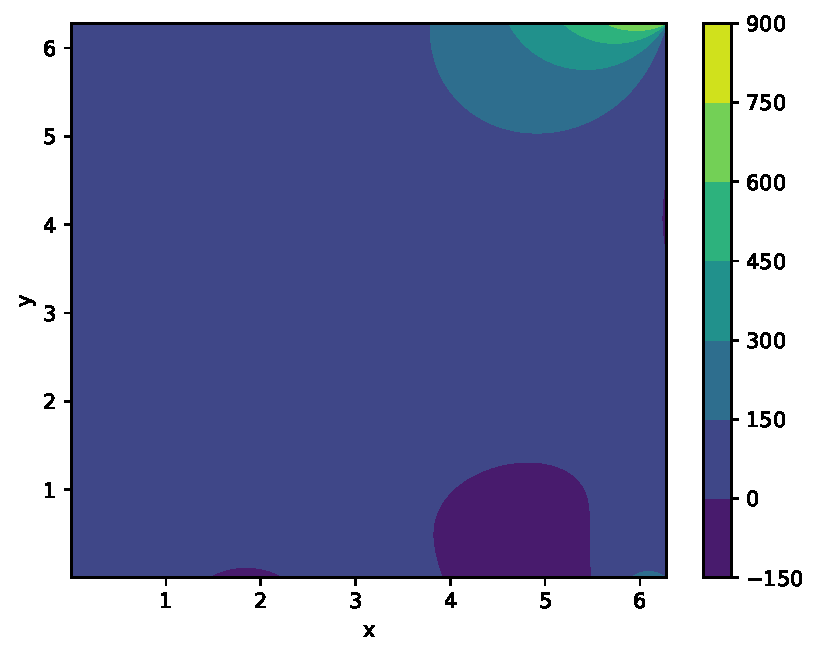
\includegraphics[width=1\textwidth]{Figures/PINN-BO/heat_py_pde_1000_test_2.pdf}
%         \caption{Solution of Temperature Equation with boundary conditions 2}
%         \label{fig:heat_2_dist}
%     \end{subfigure}
%     \hfill
%     \begin{subfigure}[b]{0.3\textwidth}
%         \centering
%         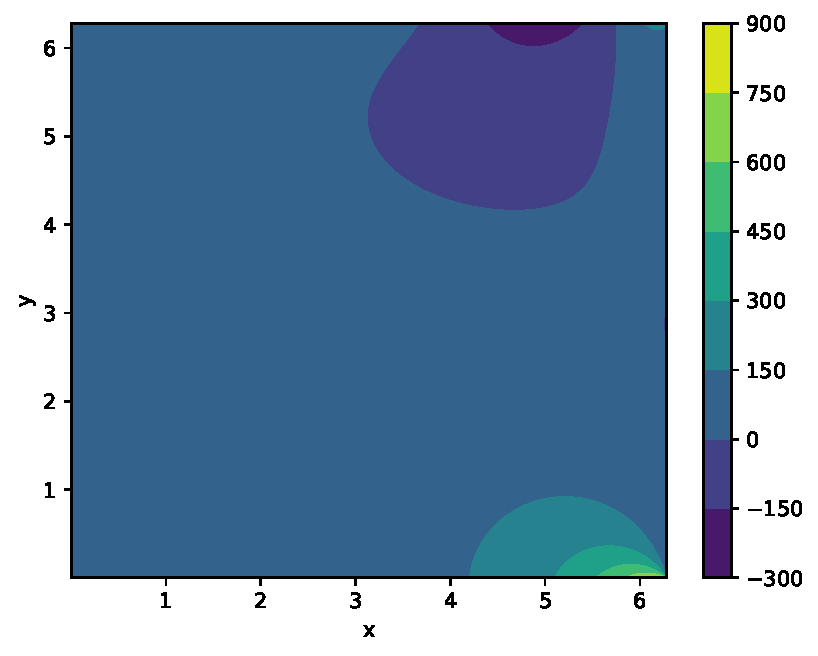
\includegraphics[width=\textwidth]{Figures/PINN-BO/heat_py_pde_1000_test_3.pdf}
%         \caption{Solution of Temperature Equation with boundary conditions 3}
%         \label{fig:heat_3_dist}
%     \end{subfigure}
%     \caption{The figures depict the solutions for temperature distributions governed by the heat equation, with each figure corresponding to a specific tuple of boundary conditions described in Section \ref{section:pinn-bo_experiments_2d_laplace}. It is evident that the region with the highest temperature is relatively small in comparison to the entire domain.}
%     \label{fig:heat_dist}
% \end{figure}

% We conducted temperature optimization by identifying the locations $(x,y)$ where the temperature reaches its maximum. As illustrated in Figure \ref{fig:heat_dist}, the area with high temperatures is relatively small in comparison to the regions with medium or low temperatures. For each baseline, we performed the optimization process 10 times, computing the average results. The comparative outcomes are presented in Figure \ref{fig:heat_opt}. 
% \begin{figure}[ht]
%     \centering
%     \begin{subfigure}[b]{0.3\textwidth}
%         \centering
%     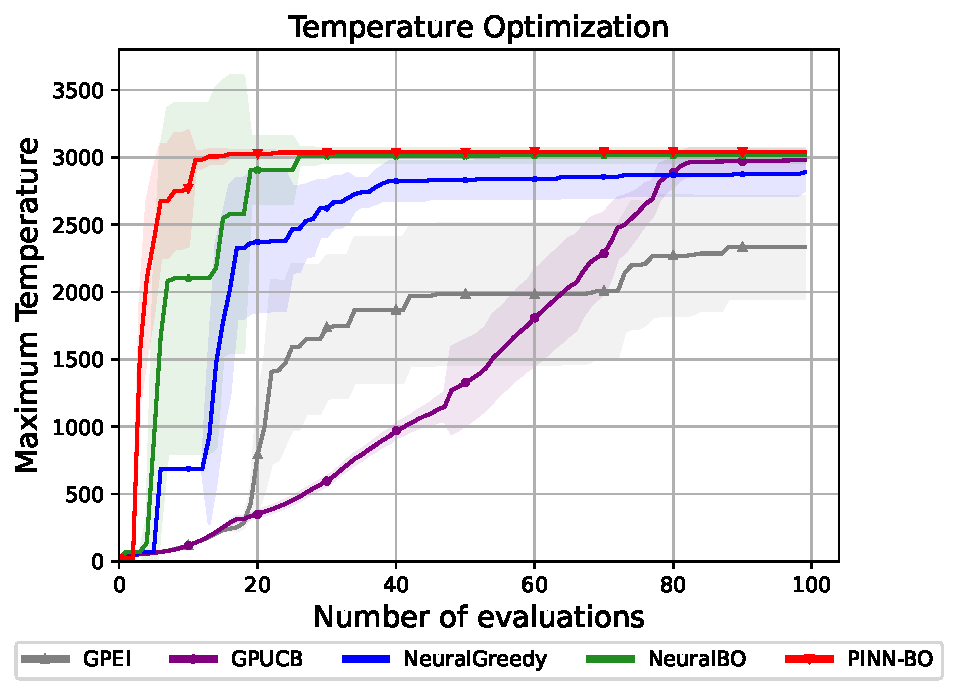
\includegraphics[width=\textwidth]{Figures/PINN-BO/Heat_dim_2_bc1.pdf}
%         \caption{Temperature Optimization in case of boundary conditions 1}
%  \label{fig:heat_1_opt}
%     \end{subfigure}
%     \hfill
%     \begin{subfigure}[b]{0.3\textwidth}
%         \centering
%         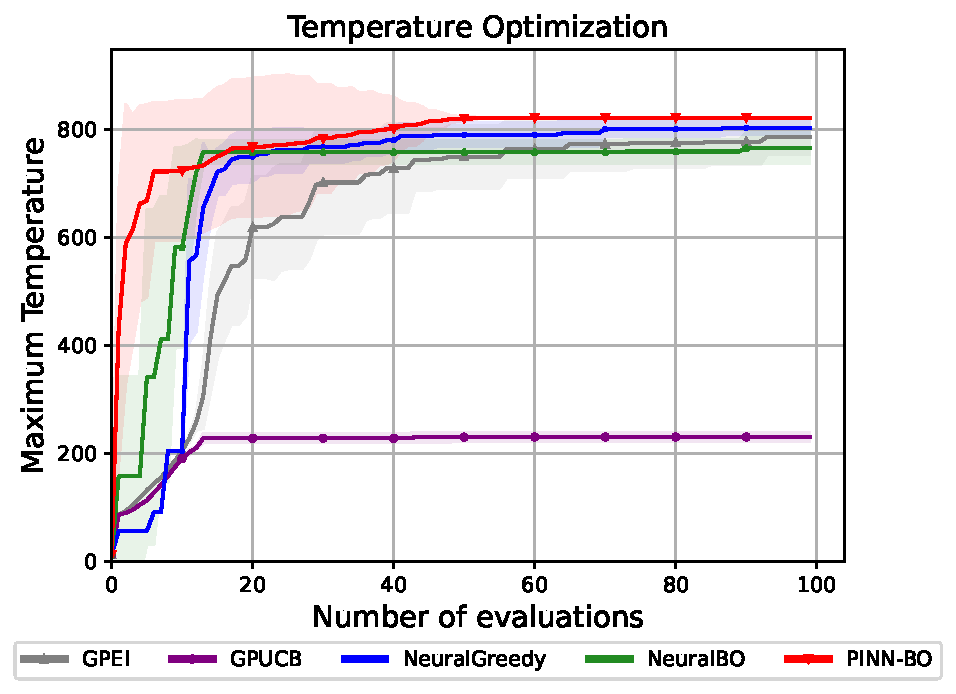
\includegraphics[width=1\textwidth]{Figures/PINN-BO/Heat_dim_2_bc2.pdf}
%         \caption{Temperature Optimization in case of boundary conditions 2}
%         \label{fig:heat_2_opt}
%     \end{subfigure}
%     \hfill
%     \begin{subfigure}[b]{0.3\textwidth}
%         \centering
%         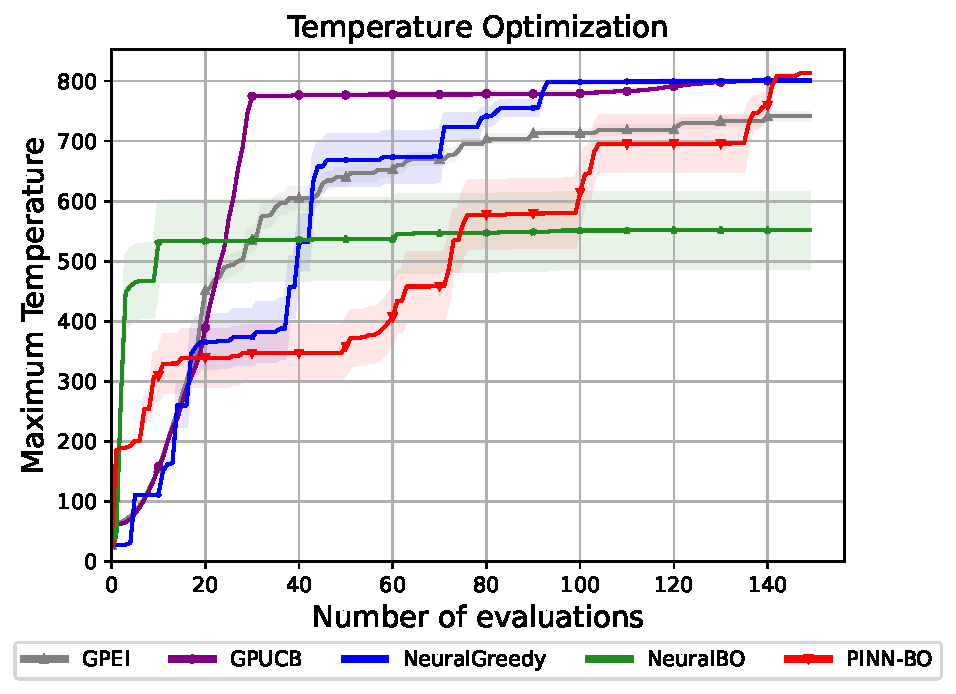
\includegraphics[width=\textwidth]{Figures/PINN-BO/Heat_dim_2_bc3.pdf}
%         \caption{Temperature Optimization in case of boundary conditions 3}
%         \label{fig:heat_3_opt}
%     \end{subfigure}
%     \caption{The figure shows the temperature optimization results of our PINN-BO and other baselines. For all three cases with different positions of maximum temperature, our PINN-BO performs better than all other baselines.}
%     \label{fig:heat_opt}
% \end{figure}


% \subsubsection{Optimizing Beam Displacement}
% We showcase the benchmark optimization outcomes obtained through our proposed method, PINN-BO, and the baseline approaches, addressing the task of minimizing the deflection of a non-uniform Euler-Bernoulli beam. The governing differential equation describing the behavior of a non-uniform Euler-Bernoulli beam is provided below: 
% \begin{equation*}
%     \frac{d^2}{dx^2} \left( EI(x) \frac{d^2 w(x)}{dx^2} \right) = q(x),
% \end{equation*}
% where
% $EI(x)$ represents the flexural rigidity of the beam, which can vary with position $x$, and $w(x)$ represents the vertical displacement of the beam at position $x$ and 
% $q(x)$ represents the distributed or concentrated load applied to the beam. 
% In our implementation, we consider the detailed expression of $EI(x)$ and $q(x)$ as follows:
% \begin{align*}
%     EI(x) &= \frac{e^x}{\rho(x)},\\
%     \rho(x) &= 2.4 x - 64 \pi^{2} e^{4 x} \sin{\left(4 \pi e^{2 x} \right)} - 396 e^{2 x} \sin{\left(20 x \right)} \\
%     &+ 80 e^{2 x} \cos{\left(20 x \right)} + 16 \pi e^{2 x} \cos{\left(4 \pi e^{2 x} \right)} + 0.4
% \end{align*}
% We employed the Finite Difference Method (FDM) to solve the non-uniform Euler-Bernoulli beam equation. It's crucial to note that this step is solely for generating observations at each input point. Despite obtaining this solution, our methods and all baseline techniques continue to treat this solution as a black-box function, accessing observations solely through querying. In Figure \ref{fig:beam_illustration}, the displacement values $w(x)$ for $x \in (0,1)$ are illustrated. The optimization results for both our PINN-BO and the other baseline methods are presented in Figure \ref{fig:beam_opt}.

% \begin{figure}[ht]
%     \centering
%     \begin{subfigure}[b]{0.44\textwidth}
%         \centering
%     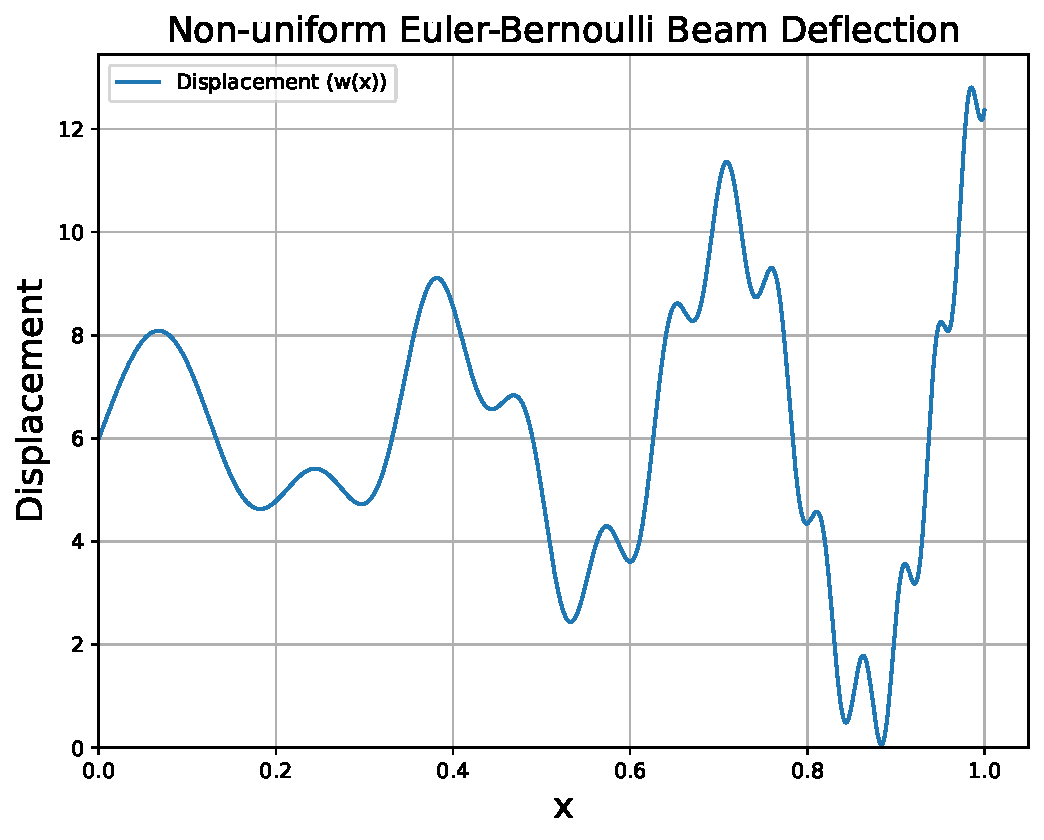
\includegraphics[width=\textwidth]{Figures/PINN-BO/beam.pdf}
%     \caption{Displacement of non-uniform Euler beam}
%      \label{fig:beam_illustration}
%     \end{subfigure}
%     \hfill
%     \begin{subfigure}[b]{0.49\textwidth}
%         \centering
%         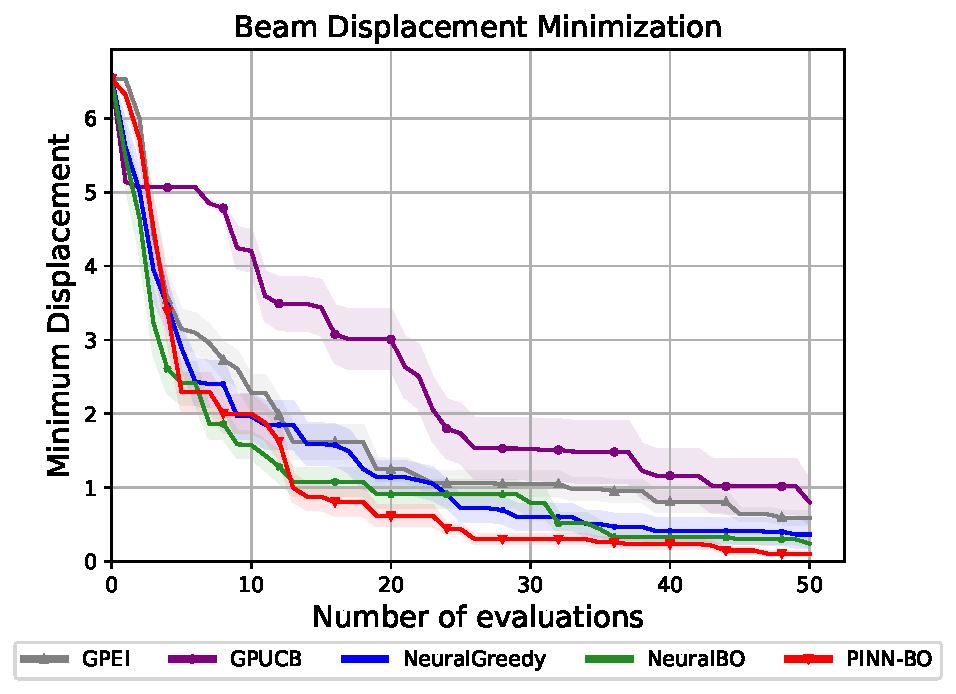
\includegraphics[width=1\textwidth]{Figures/PINN-BO/BeamDeflection_dim_1.pdf}
%         \caption{Displacement Optimization of non-uniform Euler beam}
%         \label{fig:beam_opt}
%     \end{subfigure}
%     \caption{Displacement of a Non-uniform Euler Beam and minimum displacement found by our PINN-BO and the other baselines. The left panel illustrates the natural displacement profile of the non-uniform Euler beam under given loads $q(x)$,  flexural rigidity $EI(x)$, and boundary conditions. The right panel depicts the optimized position on the beam where the displacement is minimized, highlighting the location where the structural response is at its lowest. }
%     \label{fig:beam}
% \end{figure}
\section{Proof of Theoretical Analysis in Chapter \ref{chap:pinn-bo}}
\label{section:pinn-bo_appendix}

\subsection{Proof of Lemma \ref{lemma:pinn-bo_PINN_mean_cov}}
In this section, we present the detailed proof of Lemma \ref{lemma:pinn-bo_PINN_mean_cov} in Chapter \ref{chap:pinn-bo}. Before going to the proof, we repeat Lemma \ref{lemma:pinn-bo_PINN_mean_cov} here:
\PinnMeanCov*

% \noindent \textbf{To prove Lemma \ref{lemma:pinn-bo_PINN_mean_cov}, we need the following lemma:}





\begin{proof} [Proof of Lemma \ref{lemma:pinn-bo_PINN_mean_cov}]
From Corollary \ref{corollary:pinn-bo_PINN_GP_func}, the priors for values of both $f$ and $g$ follow a joint Gaussian distribution with kernel $\mathbf{K}_\mathrm{NTK-PINN}$. Let $\mathbf{K_x}$ be the NTK matrix between point $\mathbf{x}$ and all training data: $\mathbf{K}_x = \begin{bmatrix}
        \Sigma_a & \Sigma_b \\
        \Sigma_c & \Sigma_d
    \end{bmatrix} =\begin{bmatrix}
         \boldsymbol{\Phi}_t \phi(\mathbf{x}) & 
         \boldsymbol{\Phi}_t \omega(\mathbf{x}) \\
         \boldsymbol{\Omega}_r\phi(\mathbf{x}) &
          \boldsymbol{\Omega}_r  \omega(\mathbf{x})  \end{bmatrix}$. 
Then the posterior of $f$ and $g$ evaluated at an input $\mathbf{x}$ will be a Gaussian distribution with mean and variance functions:
\paragraph{Mean function:}
\begin{align*}
    &\;\;\;\; \begin{bmatrix}
        \mu_t^f(\mathbf{x})\\
        \mu_t^g(\mathbf{x}) 
    \end{bmatrix} = \mathbf{K}_\mathbf{x} ^\top \mathbf{\widehat{K}}_\mathrm{PINN}^{-1} \begin{bmatrix}
        \mathbf{Y}_t \\
        \mathbf{U}_r
    \end{bmatrix}
    \\
    &= \begin{bmatrix}
        \Sigma_a^\top & \Sigma_c^\top \\
        \Sigma_b^\top & \Sigma_d^\top
    \end{bmatrix} \begin{bmatrix}
        \widetilde{\mathbf{A}} & \widetilde{\mathbf{B}} \\
    \widetilde{\mathbf{C}} & \widetilde{\mathbf{D}}
    \end{bmatrix} \begin{bmatrix}
        \mathbf{Y}_t \\
        \mathbf{U}_r
    \end{bmatrix}\\
    &= \begin{bmatrix}
        \phi(\mathbf{x})^\top \boldsymbol{\Phi}_t^\top &  \phi(\mathbf{x})^\top \boldsymbol{\Omega}_r ^\top \\
        \omega(\mathbf{x})^\top \boldsymbol{\Phi}_t^\top  & \omega(\mathbf{x})^\top \boldsymbol{\Omega}_r ^\top
    \end{bmatrix} \begin{bmatrix}
        \widetilde{\mathbf{A}} & \widetilde{\mathbf{B}} \\
    \widetilde{\mathbf{C}} & \widetilde{\mathbf{D}}
    \end{bmatrix} \begin{bmatrix}
        \mathbf{Y}_t \\
        \mathbf{U}_r
    \end{bmatrix} \\
    & = \begin{bmatrix}
         \phi(\mathbf{x})^\top \boldsymbol{\Phi}_t^\top \widetilde{\mathbf{A}}\mathbf{Y}_t +  \phi(\mathbf{x})^\top \boldsymbol{\Omega}_r ^\top  \widetilde{\mathbf{C}}\mathbf{Y}_t  + \phi(\mathbf{x})^\top \boldsymbol{\Phi}_t^\top \widetilde{\mathbf{B}} \mathbf{U}_r   +  \phi(\mathbf{x})^\top \boldsymbol{\Omega}_r ^\top  \widetilde{\mathbf{D}} \mathbf{U}_r \\
         \omega(\mathbf{x})^\top \boldsymbol{\Phi}_t^\top \widetilde{\mathbf{A}} \mathbf{Y}_t +  \omega(\mathbf{x})^\top \boldsymbol{\Omega}_r ^\top  \widetilde{\mathbf{C}} \mathbf{Y}_t  +\omega(\mathbf{x})^\top \boldsymbol{\Phi}_t^\top \widetilde{\mathbf{B}} \mathbf{U}_r  +  \omega(\mathbf{x})^\top \boldsymbol{\Omega}_r ^\top  \widetilde{\mathbf{D}} \mathbf{U}_r
    \end{bmatrix}
        \\
         &=\phi(\mathbf{x})^\top \boldsymbol{\xi}_t^\top \mathbf{\widehat{K}}_\mathrm{PINN}^{-1} \begin{bmatrix}
         \mathbf{Y}_t \\
         \mathbf{U}_r\end{bmatrix}
\end{align*}

\paragraph{Variance function:}
Let $\mathbf{K}_{\mathbf{xx}} = \begin{bmatrix}
\langle \phi(\mathbf{x}), \phi(\mathbf{x}) \rangle & \langle \phi(\mathbf{x}), \omega(\mathbf{x}) \rangle \\
\langle \omega(\mathbf{x}), \phi(\mathbf{x}) \rangle & \langle \omega(\mathbf{x}), \omega(\mathbf{x}) \rangle
\end{bmatrix}$, then we have the posterior covariance matrix of $f$ and $g$ at input $\mathbf{x}$ is:
\begin{align*}
    &\begin{bmatrix}
    \mathrm{Cov}_f(\mathbf{x}) & \mathrm{Cov}_{fg}(\mathbf{x}) \\
    \mathrm{Cov}_{gf}(\mathbf{x}) & \mathrm{Cov}_g(\mathbf{x})
\end{bmatrix}  \\
&= \nu_t^2 \left(\mathbf{K}_{\mathbf{xx}} - \mathbf{K_x}^\top \mathbf{\widehat{K}}_\mathrm{PINN}^{-1} \mathbf{K_x} \right) \\
&= \nu_t^2   \begin{bmatrix}
\langle \phi(\mathbf{x}), \phi(\mathbf{x}) \rangle & \langle \phi(\mathbf{x}), \omega(\mathbf{x}) \rangle \notag \\
\langle \omega(\mathbf{x}), \phi(\mathbf{x}) \rangle & \langle \omega(\mathbf{x}), \omega(\mathbf{x}) \rangle
\end{bmatrix} - \nu_t^2
\begin{bmatrix}
        \Sigma_a^\top& \Sigma_c^\top \\
        \Sigma_b^\top & \Sigma_d^\top
\end{bmatrix} \begin{bmatrix}
    \widetilde{\mathbf{A}} & \widetilde{\mathbf{B}} \\
    \widetilde{\mathbf{C}} & \widetilde{\mathbf{D}}
        \end{bmatrix}  \begin{bmatrix}
                            \Sigma_a & \Sigma_b \\
                            \Sigma_c & \Sigma_d
                        \end{bmatrix}  \\
\end{align*}
Therefore, 
\begin{align*}
\mathrm{Cov}_f(\mathbf{x}) & = \nu_t^2 \langle \phi(\mathbf{x}),  \phi(\mathbf{x}) \rangle - \nu_t^2(\Sigma_a^\top \widetilde{\mathbf{A}}\Sigma_a + \Sigma_c^\top \widetilde{\mathbf{C}}\Sigma_c + \Sigma_a^\top \widetilde{\mathbf{B}}\Sigma_a + \Sigma_c^\top \widetilde{\mathbf{D}}\Sigma_c) \\
        & = \nu_t^2 \langle \phi(\mathbf{x}),  \phi(\mathbf{x}) \rangle - \nu_t^2 \begin{bmatrix}
            \Sigma_a^\top  & \Sigma_c^\top
        \end{bmatrix}
        \begin{bmatrix}
    \widetilde{\mathbf{A}} & \widetilde{\mathbf{B}} \\
    \widetilde{\mathbf{C}} & \widetilde{\mathbf{D}}
        \end{bmatrix} \begin{bmatrix}
            \Sigma_a \\ \Sigma_c
        \end{bmatrix}  \\
        &= \nu_t^2 \langle \phi(\mathbf{x}),  \phi(\mathbf{x}) \rangle - \nu_t^2\begin{bmatrix}
            \phi(\mathbf{x})^\top \boldsymbol{\Phi}_t^\top & \phi(\mathbf{x})^\top \boldsymbol{\Omega}_r^\top
        \end{bmatrix}  \begin{bmatrix}
    \widetilde{\mathbf{A}} & \widetilde{\mathbf{B}} \\
    \widetilde{\mathbf{C}} & \widetilde{\mathbf{D}}
        \end{bmatrix} \begin{bmatrix} \boldsymbol{\Phi}_t \phi(\mathbf{x}) \\ \boldsymbol{\Omega}_r \phi(\mathbf{x})  \end{bmatrix}  \\
        &= \nu_t^2 \langle \phi(\mathbf{x}),  \phi(\mathbf{x}) \rangle - \nu_t^2\phi(\mathbf{x})^\top \boldsymbol{\xi}_t^\top \mathbf{\widehat{K}}_\mathrm{PINN}^{-1} \boldsymbol{\xi}_t \phi(\mathbf{x})\\
        &= \nu_t^2 (\sigma_t^f)^2(\mathbf{x})
\end{align*}
\end{proof}

\subsection{Proof of Lemma \ref{lemma:pinn-bo_interaction_information_formula}}
Before going to the proof, we repeat Lemma \ref{lemma:pinn-bo_interaction_information_formula}
\InteractionInformation*


% \noindent \textbf{To prove Lemma \ref{lemma:pinn-bo_interaction_information_formula}, we need to prove the following technical lemma:}



\begin{proof}[Proof of Lemma \ref{lemma:pinn-bo_interaction_information_formula}]
By definition, we have $I (f; \mathbf{Y}_t; \mathbf{U}_r) = I(f; \mathbf{Y}_t) - I (f; \mathbf{Y}_t \rvert \mathbf{U}_r)$. We start the proof by calculating $I (f; \mathbf{Y}_t \rvert \mathbf{U}_r)$.

Using the properties of \acp{gp}, given a set of sampling points $\mathcal{D}_t\subset \mathcal{D}$, we have that $f, \mathbf{Y}_t, \mathbf{U}_r$ are jointly Gaussian:
\begin{align} 
\label{Eqn:joint_gauss_3_variables}
\begin{pmatrix}
    f \\
    \mathbf{Y}_t \\
    \mathbf{U}_r
\end{pmatrix} \sim \mathcal{N} \left(\mathbf{0}, \nu_t^2 \begin{bmatrix}
    \mathbf{K}_{uu} & \mathbf{K}_{uu} & \mathbf{K}_{ur} \\
    \mathbf{K}_{uu} & \mathbf{K}_{uu} + \lambda_1 \mathbf{I} & \mathbf{K}_{ur} \\
    \mathbf{K}_{ru} & \mathbf{K}_{uu} & \mathbf{K}_{rr} + \lambda_2 \mathbf{I}
\end{bmatrix} \right)   
\end{align} 
Then, we have:

\begin{align}
    \textup{Cov}(f \rvert \mathbf{U}_r) &=  \nu_t^2 \left[ \mathbf{K}_{uu} - \mathbf{K}_{ur}(\mathbf{K}_{rr}+ \lambda_2\mathbf{I})^{-1} \mathbf{K}_{ru} \right] \nonumber
        \\
        &= \nu_t^2 \left[\boldsymbol{\Phi}_t \boldsymbol{\Phi}_t^\top - \boldsymbol{\Phi}_t\boldsymbol{\Omega}_r^\top (\boldsymbol{\Omega}_r\boldsymbol{\Omega}_r^\top + \lambda_2\mathbf{I})^{-1} \boldsymbol{\Omega}_r\boldsymbol{\Phi}_t^\top \right] \nonumber
        \\
        &= \nu_t^2 \left[\boldsymbol{\Phi}_t\boldsymbol{\Phi}_t^\top - \boldsymbol{\Phi}_t\left[\mathbf{I} - \lambda_2(\boldsymbol{\Omega}_r\boldsymbol{\Omega}_r^\top + \lambda_2\mathbf{I})^{-1}\right] \boldsymbol{\Phi}_t^\top \right] \nonumber
        \\
        &= \nu_t^2 \lambda_2 \boldsymbol{\Phi}_t (\boldsymbol{\Omega}_r^\top \boldsymbol{\Omega}_r + \lambda_2\mathbf{I})^{-1} \boldsymbol{\Phi}_t^\top \nonumber 
        \\ 
        &= \nu_t^2 \boldsymbol{\Phi}_t \left(\frac{\boldsymbol{\Omega}_r^\top \boldsymbol{\Omega}_r}{\lambda_2} + \mathbf{I}\right)^{-1} \boldsymbol{\Phi}_t^\top, \label{Eqn:covar_f_condition_on_u}  
\end{align}
and 
\begin{align}
        \textup{Cov}(f \rvert \mathbf{Y}_t; \mathbf{U}_r) &= \nu_t^2 \left(\mathbf{K}_{uu} - \begin{bmatrix}
            \mathbf{K}_{uu} & \mathbf{K}_{ur}
        \end{bmatrix} \begin{bmatrix}
            \mathbf{K}_{uu} + \lambda_1\mathbf{I} & \mathbf{K}_{ur} \\
            \mathbf{K}_{ru} & \mathbf{K}_{rr} + \lambda_2 \mathbf{I}
        \end{bmatrix}^{-1} \begin{bmatrix}
            \mathbf{K}_{uu} \\
            \mathbf{K}_{ru}
        \end{bmatrix} \right)  \nonumber
        \\
        & = \nu_t^2 (\boldsymbol{\Phi}_t \boldsymbol{\Phi}_t^\top - \boldsymbol{\Phi}_t \boldsymbol{\xi}_t^\top \mathbf{\widehat{K}}_\mathrm{PINN}^{-1} \boldsymbol{\xi}_t \boldsymbol{\Phi}_t^\top).  \label{Eqn:covar_f_condition_on_y_and_u}
\end{align}
Let $\mathbf{V} = \boldsymbol{\xi}_t^\top \mathbf{\widehat{K}}_\mathrm{PINN}^{-1} \boldsymbol{\xi}_t$, now we need to calculate $\mathbf{V}$. We have
\begin{align*}
            \mathbf{V} &= \boldsymbol{\boldsymbol{\xi}_t}^\top \mathbf{\widehat{K}}_\mathrm{PINN}^{-1} \boldsymbol{\boldsymbol{\xi}_t} 
\\
            &=\boldsymbol{\Phi}_t^\top \widetilde{\mathbf{A}}\boldsymbol{\Phi}_t + \boldsymbol{\Omega}_r^\top \widetilde{\mathbf{C}}\boldsymbol{\Phi}_t + \boldsymbol{\Phi}_t^\top \widetilde{\mathbf{B}}\boldsymbol{\Omega}_r + \boldsymbol{\Omega}_r^\top \widetilde{\mathbf{D}}\boldsymbol{\Omega}_r 
\\
            & = \boldsymbol{\Phi}_t^\top (\mathbf{P}^{-1} - \mathbf{P}^{-1}\mathbf{Q}\widetilde{\mathbf{C}})\boldsymbol{\Phi}_t + \boldsymbol{\Omega}_r^\top \widetilde{\mathbf{C}}\boldsymbol{\Phi}_t - \boldsymbol{\Phi}_t^\top \mathbf{P}^{-1}\mathbf{Q}\boldsymbol{\Omega}_r + \boldsymbol{\Omega}_r^\top \widetilde{\mathbf{D}}\boldsymbol{\Omega}_r 
\\
            & = \boldsymbol{\Phi}_t^\top \mathbf{P}^{-1}\boldsymbol{\Phi}_t - \boldsymbol{\Phi}_t^\top\mathbf{P}^{-1}\mathbf{Q}\widetilde{\mathbf{C}}\boldsymbol{\Phi}_t + \boldsymbol{\Omega}_r^\top \widetilde{\mathbf{C}}\boldsymbol{\Phi}_t - \boldsymbol{\Phi}_t^\top \mathbf{P}^{-1}\mathbf{Q}\boldsymbol{\Omega}_r + \boldsymbol{\Omega}_r^\top \widetilde{\mathbf{D}}\boldsymbol{\Omega}_r 
\\
            & = \boldsymbol{\Phi}_t^\top \mathbf{P}^{-1}\boldsymbol{\Phi}_t + (\underbrace{\boldsymbol{\Omega}_r - \boldsymbol{\Phi}_t^\top\mathbf{P}^{-1}\mathbf{Q}}_{U_1})(\widetilde{\mathbf{C}}\boldsymbol{\Phi}_t + \widetilde{\mathbf{D}}\boldsymbol{\Omega}_r) 
\\
            & = \boldsymbol{\Phi}_t^\top \mathbf{P}^{-1}\boldsymbol{\Phi}_t + (\underbrace{\boldsymbol{\Omega}_r - \boldsymbol{\Phi}_t^\top\mathbf{P}^{-1}\mathbf{Q}}_{V_1})(\underbrace{\widetilde{\mathbf{C}}\boldsymbol{\Phi}_t + \widetilde{\mathbf{D}}\boldsymbol{\Omega}_r)}_{V_2} \\
            & = \boldsymbol{\Phi}_t^\top (\boldsymbol{\Phi}_t\boldsymbol{\Phi}_t^\top+\lambda_1 \mathbf{I})^{-1} \boldsymbol{\Phi}_t + V_1V_2
\\
            & = (\boldsymbol{\Phi}_t^\top\boldsymbol{\Phi}_t+\lambda_1 \mathbf{I})^{-1} \boldsymbol{\Phi}_t^\top\boldsymbol{\Phi}_t + V_1V_2,
\end{align*}
where 
\begin{align*}
            \begin{bmatrix}
            \mathbf{P} & \mathbf{Q} \\
            \mathbf{R} & \mathbf{S}
            \end{bmatrix} & = \begin{bmatrix}
            \mathbf{K}_{uu} + \lambda_1\mathbf{I} & \mathbf{K}_{ur}  \\
            \mathbf{K}_{ru}  & \mathbf{K}_{rr} + \lambda_2\mathbf{I}
            \end{bmatrix} = \begin{bmatrix}
            \boldsymbol{\Phi}_t\boldsymbol{\Phi}_t^\top + \lambda_1\mathbf{I} & \boldsymbol{\Phi}_t \boldsymbol{\Omega}_r^\top \\
            \boldsymbol{\Omega}_r\boldsymbol{\Phi}_t^\top & \boldsymbol{\Omega}_r\boldsymbol{\Omega}_r^\top + \lambda_2 \mathbf{I}\end{bmatrix} \\
            \text{and} \begin{bmatrix}
    \widetilde{\mathbf{A}} & \widetilde{\mathbf{B}} 
\\
    \widetilde{\mathbf{C}} & \widetilde{\mathbf{D}} 
        \end{bmatrix} &=\begin{bmatrix}
            \mathbf{P} & \mathbf{Q} \\
            \mathbf{R} & \mathbf{S}
            \end{bmatrix} ^{-1}.
\end{align*}
The second equality applied the formula of block matrix inversion\footnote{The inversion of matrix $\mathbf{K} = \begin{bmatrix}
        \mathbf{P} & \mathbf{Q} \\ \mathbf{R} & \mathbf{S} 
    \end{bmatrix}$ is given as $\mathbf{K}^{-1} = \begin{bmatrix}
        \mathbf{P}^{-1} + \mathbf{P}^{-1} \mathbf{QMR}\mathbf{P}^{-1} & \mathbf{P}^{-1}\mathbf{QM} \\ -\mathbf{MR}\mathbf{P}^{-1} & \mathbf{M} 
    \end{bmatrix}$ with $\mathbf{M} = (\mathbf{S} - \mathbf{R}\mathbf{P}^{-1}\mathbf{Q})^{-1}$.}, 
    while the last equality used push-through identity. Next, we have
\begin{align*}
            \mathbf{M} &= (\mathbf{S} - \mathbf{R}\mathbf{P}^{-1}\mathbf{Q})^{-1} 
\\
            &= \left[\boldsymbol{\Omega}_r \boldsymbol{\Omega}_r^\top  + \lambda_2\mathbf{I} - \boldsymbol{\Omega}_r \boldsymbol{\Phi}_t^\top (\boldsymbol{\Phi}_t \boldsymbol{\Phi}_t ^\top+ \lambda_1\mathbf{I})^{-1} \boldsymbol{\Phi}_t \boldsymbol{\Omega}_r^\top)\right]^{-1} 
\\
            &= \left[\boldsymbol{\Omega}_r \boldsymbol{\Omega}_r^\top  + \lambda_2\mathbf{I} - \boldsymbol{\Omega}_r (\boldsymbol{\Phi}_t^\top \boldsymbol{\Phi}_t+ \lambda_1\mathbf{I})^{-1} \boldsymbol{\Phi}_t^\top \boldsymbol{\Phi}_t \right] \boldsymbol{\Omega}_r^\top)^{-1} 
\\ 
            &= \left[\boldsymbol{\Omega}_r \boldsymbol{\Omega}_r^\top  + \lambda_2\mathbf{I} - \boldsymbol{\Omega}_r \left[ \mathbf{I} - \lambda_1(\boldsymbol{\Phi}_t^\top \boldsymbol{\Phi}_t+ \lambda_1\mathbf{I})^{-1} \right] \boldsymbol{\Omega}_r^\top)\right]^{-1} 
\\ 
            &= \left[\lambda_2\mathbf{I} + \lambda_1\boldsymbol{\Omega}_r(\boldsymbol{\Phi}_t^\top \boldsymbol{\Phi}_t+ \lambda_1\mathbf{I})^{-1}\boldsymbol{\Omega}_r^\top\right]^{-1} 
\\
            &= \lambda_1^{-1} \left[\boldsymbol{\Omega}_r(\boldsymbol{\Phi}_t^\top \boldsymbol{\Phi}_t+ \lambda_1\mathbf{I})^{-1}\boldsymbol{\Omega}_r^\top + \frac{\lambda_2} {\lambda_1} \mathbf{I}\right]^{-1} 
\\
            V_1 & = \boldsymbol{\Omega}_r^\top - \boldsymbol{\Phi}_t^\top \mathbf{P}^{-1} \mathbf{Q}
\\
            & = \boldsymbol{\Omega}_r^\top - \boldsymbol{\Phi}_t^\top (\boldsymbol{\Phi}_t\boldsymbol{\Phi}_t^\top + \lambda_1\mathbf{I})^{-1} \boldsymbol{\Phi}_t \boldsymbol{\Omega}_r^\top 
\\
            &=\left[ \mathbf{I} - \boldsymbol{\Phi}_t^\top (\boldsymbol{\Phi}_t\boldsymbol{\Phi}_t^\top + \lambda_1\mathbf{I})^{-1} \boldsymbol{\Phi}_t\right] \boldsymbol{\Omega}_r^\top 
\\
            & = \left[ \mathbf{I} - (\boldsymbol{\Phi}_t^\top\boldsymbol{\Phi}_t + \lambda_1\mathbf{I})^{-1} \boldsymbol{\Phi}_t^\top\boldsymbol{\Phi}_t\right] \boldsymbol{\Omega}_r^\top 
\\
            & = \left[ \mathbf{I} - (\boldsymbol{\Phi}_t^\top\boldsymbol{\Phi}_t + \lambda_1\mathbf{I})^{-1} (\boldsymbol{\Phi}_t^\top\boldsymbol{\Phi}_t +\lambda_1 \mathbf{I} - \lambda_1 \mathbf{I})\right] \boldsymbol{\Omega}_r^\top 
\\
            & = \lambda_1(\boldsymbol{\Phi}_t^\top\boldsymbol{\Phi}_t + \lambda_1\mathbf{I})^{-1} \boldsymbol{\Omega}_r^\top 
\\
            V_2 & = \widetilde{\mathbf{C}}\boldsymbol{\Phi}_t  + \widetilde{\mathbf{D}}\boldsymbol{\Omega}_r 
\\
            & = -\mathbf{M}\mathbf{R}\mathbf{P}^{-1} + \mathbf{M}\boldsymbol{\Omega}_r 
\\
            & = \mathbf{M}(\boldsymbol{\Omega}_r - \mathbf{R}\mathbf{P}^{-1}\boldsymbol{\Phi}_t)
\\
            & = \mathbf{M}\left[\boldsymbol{\Omega}_r - \boldsymbol{\Omega}_r \boldsymbol{\Phi}_t^\top (\boldsymbol{\Phi}_t \boldsymbol{\Phi}_t^\top + \lambda_1\mathbf{I})^{-1}\boldsymbol{\Phi}_t\right] 
\\
            & = \mathbf{M}\boldsymbol{\Omega}_r \left[ \mathbf{I} - \boldsymbol{\Phi}_t^\top (\boldsymbol{\Phi}_t \boldsymbol{\Phi}_t^\top + \lambda_1\mathbf{I})^{-1}\boldsymbol{\Phi}_t\right]
\\
            & = \lambda_1 \mathbf{M} \boldsymbol{\Omega}_r (\boldsymbol{\Phi}_t^\top \boldsymbol{\Phi}_t + \lambda_1\mathbf{I})^{-1} 
\\ 
            & = \left[\boldsymbol{\Omega}_r(\boldsymbol{\Phi}_t^\top \boldsymbol{\Phi}_t+ \lambda_1\mathbf{I})^{-1}\boldsymbol{\Omega}_r^\top + \frac{\lambda_2} {\lambda_1} \mathbf{I}\right]^{-1} \boldsymbol{\Omega}_r (\boldsymbol{\Phi}_t^\top \boldsymbol{\Phi}_t + \lambda_1\mathbf{I})^{-1}
\end{align*}
Then we have, 
    \begin{align*}
            \mathbf{V} &= \boldsymbol{\boldsymbol{\xi}_t}^\top \mathbf{\widehat{K}}_\mathrm{PINN}^{-1} \boldsymbol{\boldsymbol{\xi}_t}  
            \\
            & = (\boldsymbol{\Phi}_t^\top\boldsymbol{\Phi}_t+\lambda_1 \mathbf{I})^{-1} \boldsymbol{\Phi}_t^\top\boldsymbol{\Phi}_t + V_1V_2
            \\
            & = (\boldsymbol{\Phi}_t^\top\boldsymbol{\Phi}_t+\lambda_1 \mathbf{I})^{-1} \boldsymbol{\Phi}_t^\top\boldsymbol{\Phi}_t + \lambda_1(\boldsymbol{\Phi}_t^\top\boldsymbol{\Phi}_t + \lambda_1\mathbf{I})^{-1} \boldsymbol{\Omega}_r^\top \notag \\
            &  \;\;\;\;\; \cdot \left[\boldsymbol{\Omega}_r(\boldsymbol{\Phi}_t^\top \boldsymbol{\Phi}_t+ \lambda_1\mathbf{I})^{-1}\boldsymbol{\Omega}_r^\top + \frac{\lambda_2} {\lambda_1} \mathbf{I}\right]^{-1} \boldsymbol{\Omega}_r (\boldsymbol{\Phi}_t^\top \boldsymbol{\Phi}_t + \lambda_1\mathbf{I})^{-1} 
            \\
            &= \mathbf{I} - \lambda_1(\boldsymbol{\Phi}_t^\top\boldsymbol{\Phi}_t+\lambda_1 \mathbf{I})^{-1} + \lambda_1(\boldsymbol{\Phi}_t^\top\boldsymbol{\Phi}_t + \lambda_1\mathbf{I})^{-1} \boldsymbol{\Omega}_r^\top \notag \\
            & \;\;\;\;\;   \cdot \left[\boldsymbol{\Omega}_r(\boldsymbol{\Phi}_t^\top \boldsymbol{\Phi}_t+ \lambda_1\mathbf{I})^{-1}\boldsymbol{\Omega}_r^\top + \frac{\lambda_2} {\lambda_1} \mathbf{I}\right]^{-1} \boldsymbol{\Omega}_r (\boldsymbol{\Phi}_t^\top \boldsymbol{\Phi}_t + \lambda_1\mathbf{I})^{-1} 
            \\
            &  = \mathbf{I} -  \lambda_1(\boldsymbol{\Phi}_t^\top\boldsymbol{\Phi}_t+\lambda_1 \mathbf{I})^{-1} \\ \notag
            \\ 
            & \;\;\;\;\;    \cdot \left[\mathbf{I} - \boldsymbol{\Omega}_r^\top \left(\boldsymbol{\Omega}_r(\boldsymbol{\Phi}_t^\top \boldsymbol{\Phi}_t+ \lambda_1\mathbf{I})^{-1}\boldsymbol{\Omega}_r^\top+\frac{\lambda_2} {\lambda_1} \mathbf{I}\right)^{-1} \boldsymbol{\Omega}_r (\boldsymbol{\Phi}_t^\top\boldsymbol{\Phi}_t+\lambda_1 \mathbf{I})^{-1} \right]
            \\
            & = \mathbf{I} -  \lambda_1(\boldsymbol{\Phi}_t^\top\boldsymbol{\Phi}_t+\lambda_1 \mathbf{I})^{-1} \\ \notag 
            \\
            & \;\;\;\;\; \cdot \left[\mathbf{I} -  \left(\boldsymbol{\Omega}_r^\top\boldsymbol{\Omega}_r(\boldsymbol{\Phi}_t^\top \boldsymbol{\Phi}_t+ \lambda_1\mathbf{I})^{-1}+\frac{\lambda_2} {\lambda_1} \mathbf{I}\right)^{-1} \boldsymbol{\Omega}_r^\top\boldsymbol{\Omega}_r (\boldsymbol{\Phi}_t^\top\boldsymbol{\Phi}_t+\lambda_1 \mathbf{I})^{-1}\right] \\ 
            & = \mathbf{I} -  \lambda_1(\boldsymbol{\Phi}_t^\top\boldsymbol{\Phi}_t+\lambda_1 \mathbf{I})^{-1} \\ \notag 
            \\
            & \;\;\;\;\; \cdot \left[\mathbf{I} -  \mathbf{I} + \frac{\lambda_2}{\lambda_1}\left(\boldsymbol{\Omega}_r^\top\boldsymbol{\Omega}_r(\boldsymbol{\Phi}_t^\top \boldsymbol{\Phi}_t+ \lambda_1\mathbf{I})^{-1}+\frac{\lambda_2} {\lambda_1} \mathbf{I}\right)^{-1} \right] \\ 
            & = \mathbf{I} - \lambda_2 (\boldsymbol{\Phi}_t^\top \boldsymbol{\Phi}_t+ \lambda_1\mathbf{I})^{-1}\left(\boldsymbol{\Omega}_r^\top\boldsymbol{\Omega}_r(\boldsymbol{\Phi}_t^\top \boldsymbol{\Phi}_t+ \lambda_1\mathbf{I})^{-1}+\frac{\lambda_2} {\lambda_1} \mathbf{I}\right)^{-1} \\
            & =\mathbf{I} - \lambda_2 \left(\boldsymbol{\Omega}_r^\top\boldsymbol{\Omega}_r+\frac{\lambda_2} {\lambda_1} (\boldsymbol{\Phi}_t^\top \boldsymbol{\Phi}_t+ \lambda_1\mathbf{I})\right)^{-1} \\
            & =\mathbf{I} - \lambda_2 \left(\boldsymbol{\Omega}_r^\top\boldsymbol{\Omega}_r+\frac{\lambda_2} {\lambda_1} \boldsymbol{\Phi}_t^\top \boldsymbol{\Phi}_t+ \lambda_2 \mathbf{I}\right)^{-1}  
    \end{align*}
In conclusion, we have 
\begin{align}
        \boldsymbol{\xi}_t^\top \mathbf{\widehat{K}}_\mathrm{PINN}^{-1} \boldsymbol{\xi}_t &= \mathbf{I} - \lambda_2 \left(\boldsymbol{\Omega}_r^\top\boldsymbol{\Omega}_r+\frac{\lambda_2} {\lambda_1} \boldsymbol{\Phi}_t^\top \boldsymbol{\Phi}_t+ \lambda_2 \mathbf{I}\right)^{-1} \nonumber
        \\
        &= \mathbf{I} -  \left(\frac{\boldsymbol{\Omega}_r^\top\boldsymbol{\Omega}_r}{\lambda_2}+\frac{\boldsymbol{\Phi}_t^\top \boldsymbol{\Phi}_t} {\lambda_1} + \mathbf{I}\right)^{-1}. \label{Eqn:xi_t-K-xi} 
\end{align}
Replace Eqn. \eqref{Eqn:xi_t-K-xi} to the expression of $\textup{Cov}(f_t \rvert \mathbf{Y}_t; \mathbf{U}_r)$ in Eqn. \eqref{Eqn:covar_f_condition_on_y_and_u}, we have: 

\begin{equation}
\label{Eqn:covar_f_condition_on_y_and_u_final}
    \textup{Cov}(f \rvert \mathbf{Y}_t; \mathbf{U}_r) = \nu_t^2\boldsymbol{\Phi}_t \left(\frac{\boldsymbol{\Omega}_r^\top\boldsymbol{\Omega}_r}{\lambda_2}+\frac{\boldsymbol{\Phi}_t^\top \boldsymbol{\Phi}_t} {\lambda_1} + \mathbf{I}\right)^{-1} \boldsymbol{\Phi}_t^\top
\end{equation}
Combining the expression of $\textup{Cov}(f\rvert \mathbf{U}_r)$ in Eqn. \eqref{Eqn:covar_f_condition_on_u} with Eqn. \eqref{Eqn:covar_f_condition_on_y_and_u_final}, with $H$ is the entropy function, we have:
\begin{align}
     & I(f;\mathbf{Y}_t \rvert \mathbf{U}_r)  \nonumber
\\
     &= H(f \rvert \mathbf{U}_r) - H(f \rvert \mathbf{Y}_t; \mathbf{U}_r)  \nonumber
\\
     & = \frac{1}{2}\log\det (\textup{Cov}(f \rvert \mathbf{U}_r)) - \frac{1}{2}\log\det (\textup{Cov}(f \rvert \mathbf{Y}_t;  \mathbf{U}_r)) \nonumber
\\
     & = \frac{1}{2}\log \det (\nu_t^2\boldsymbol{\Phi}_t \left(\frac{\boldsymbol{\Omega}_r^\top \boldsymbol{\Omega}_r}{\lambda_2} + \mathbf{I}\right)^{-1} \boldsymbol{\Phi}_t^\top) \nonumber 
\\
     & - \frac{1}{2}\log\det (\nu_t^2\boldsymbol{\Phi}_t \left(\frac{\boldsymbol{\Omega}_r^\top\boldsymbol{\Omega}_r}{\lambda_2}+\frac{\boldsymbol{\Phi}_t^\top \boldsymbol{\Phi}_t} {\lambda_1} + \mathbf{I}\right)^{-1} \boldsymbol{\Phi}_t^\top) \nonumber
\\
     &= \frac{1}{2} \log \frac{\det(\boldsymbol{\Phi}_t \left(\frac{\boldsymbol{\Omega}_r^\top \boldsymbol{\Omega}_r}{\lambda_2} + \mathbf{I}\right)^{-1} \boldsymbol{\Phi}_t^\top)}{\det(\boldsymbol{\Phi}_t \left(\frac{\boldsymbol{\Omega}_r^\top\boldsymbol{\Omega}_r}{\lambda_2}+\frac{\boldsymbol{\Phi}_t^\top \boldsymbol{\Phi}_t} {\lambda_1} + \mathbf{I}\right)^{-1} \boldsymbol{\Phi}_t^\top)}, \label{Eqn:conditional_information_f_and_Yt_give_Ur}
\end{align}
Then we have 
\begin{align}
    & I (f; \mathbf{Y}_t; \mathbf{U}_r) \nonumber 
\\
    & =  I(f; \mathbf{Y}_t) - I (f; \mathbf{Y}_t \rvert \mathbf{U}_r) \nonumber
\\
        &= \frac{1}{2} \log \det (\frac{\boldsymbol{\Phi}_t\boldsymbol{\Phi}_t^\top}{\lambda_1} +\mathbf{I}) - \frac{1}{2} \log \frac{\det(\boldsymbol{\Phi}_t \left(\frac{\boldsymbol{\Omega}_r^\top \boldsymbol{\Omega}_r}{\lambda_2} + \mathbf{I}\right)^{-1} \boldsymbol{\Phi}_t^\top)}{\det(\boldsymbol{\Phi}_t \left(\frac{\boldsymbol{\Omega}_r^\top\boldsymbol{\Omega}_r}{\lambda_2}+\frac{\boldsymbol{\Phi}_t^\top \boldsymbol{\Phi}_t} {\lambda_1} + \mathbf{I}\right)^{-1} \boldsymbol{\Phi}_t^\top)} \nonumber
\\
        & = \frac{1}{2}\log \frac{ \det (\frac{\boldsymbol{\Phi}_t\boldsymbol{\Phi}_t^\top}{\lambda_1} +\mathbf{I})
        \det(\boldsymbol{\Phi}_t \left(\frac{\boldsymbol{\Omega}_r^\top\boldsymbol{\Omega}_r}{\lambda_2}+\frac{\boldsymbol{\Phi}_t^\top \boldsymbol{\Phi}_t} {\lambda_1} + \mathbf{I}\right)^{-1} \boldsymbol{\Phi}_t^\top)
        }{\det(\boldsymbol{\Phi}_t \left(\frac{\boldsymbol{\Omega}_r^\top \boldsymbol{\Omega}_r}{\lambda_2} + \mathbf{I}\right)^{-1} \boldsymbol{\Phi}_t^\top)}  \nonumber
\\ 
        & = \frac{1}{2}\log \frac{\det[\left(\frac{\boldsymbol{\Phi}_t\boldsymbol{\Phi}_t^\top}{\lambda_1} +\mathbf{I}\right) \boldsymbol{\Phi}_t \left(\frac{\boldsymbol{\Omega}_r^\top\boldsymbol{\Omega}_r}{\lambda_2}+\frac{\boldsymbol{\Phi}_t^\top \boldsymbol{\Phi}_t} {\lambda_1} + \mathbf{I}\right)^{-1}\boldsymbol{\Phi}_t^\top]}
        {\det[ \boldsymbol{\Phi}_t \left(\frac{\boldsymbol{\Omega}_r^\top \boldsymbol{\Omega}_r}{\lambda_2} + \mathbf{I}\right)^{-1} \boldsymbol{\Phi}_t^\top]} \nonumber
\\ 
        & = \frac{1}{2}\log \frac{
        \det[\boldsymbol{\Phi}_t \left(\frac{\boldsymbol{\Phi}_t^\top\boldsymbol{\Phi}_t}{\lambda_1} +\mathbf{I}\right)  \left(\frac{\boldsymbol{\Omega}_r^\top\boldsymbol{\Omega}_r}{\lambda_2}+\frac{\boldsymbol{\Phi}_t^\top \boldsymbol{\Phi}_t} {\lambda_1} + \mathbf{I}\right)^{-1}\boldsymbol{\Phi}_t^\top]}
        {\det[ \boldsymbol{\Phi}_t \left(\frac{\boldsymbol{\Omega}_r^\top \boldsymbol{\Omega}_r}{\lambda_2} + \mathbf{I}\right)^{-1} \boldsymbol{\Phi}_t^\top]} \nonumber
\\
        & = \frac{1}{2}\log \frac{
        \det[\boldsymbol{\Phi}_t  \left(\frac{\boldsymbol{\Omega}_r^\top \boldsymbol{\Omega}_r}{\lambda_2} \left(\frac{\boldsymbol{\Phi}_t^\top\boldsymbol{\Phi}_t}{\lambda_1} +\mathbf{I}\right)^{-1} + \mathbf{I}\right)^{-1}\boldsymbol{\Phi}_t^\top]}
        {\det[ \boldsymbol{\Phi}_t \left(\frac{\boldsymbol{\Omega}_r^\top \boldsymbol{\Omega}_r}{\lambda_2} + \mathbf{I}\right)^{-1} \boldsymbol{\Phi}_t^\top]} \label{Eqn:det_division}
\\
        &= \frac{1}{2}\log \frac{\det\left(\frac{\boldsymbol{\Omega}_r^\top \boldsymbol{\Omega}_r}{\lambda_2} \left(\frac{\boldsymbol{\Phi}_t^\top\boldsymbol{\Phi}_t}{\lambda_1} +\mathbf{I}\right)^{-1} + \mathbf{I}\right)^{-1}}{\det (\frac{\boldsymbol{\Omega}_r^\top\boldsymbol{\Omega}_r}{\lambda_2} + \mathbf{I})^{-1}} \nonumber
\\
        & = \frac{1}{2}\log \frac{\det (\frac{\boldsymbol{\Omega}_r^\top\boldsymbol{\Omega}_r}{\lambda_2} + \mathbf{I})}{\det\left(\frac{\boldsymbol{\Omega}_r^\top \boldsymbol{\Omega}_r}{\lambda_2} \left(\frac{\boldsymbol{\Phi}_t^\top\boldsymbol{\Phi}_t}{\lambda_1} +\mathbf{I}\right)^{-1} + \mathbf{I}\right)} \nonumber
\\ 
        & = \frac{1}{2}  \log \left(\frac{\det(\frac{\boldsymbol{\Phi}_t^\top \boldsymbol{\Phi}_t}{\lambda_1} + \mathbf{I})\det(\frac{\boldsymbol{\Omega}_r^\top \boldsymbol{\Omega}_r}{\lambda_2} + \mathbf{I})}{\det(\frac{\boldsymbol{\Phi}_t^\top \boldsymbol{\Phi}_t}{\lambda_1} + \frac{\boldsymbol{\Omega}_r^\top \boldsymbol{\Omega}_r}{\lambda_2} + \mathbf{I})} \right), \nonumber
\end{align}
where Eqn. \eqref{Eqn:det_division} is resulted from technical Lemma \ref{lemma:pinn-bo_det_division}. 
\end{proof}
\subsection{Proof of Lemma \ref{lemma:pinn-bo_confidence_bound}}
Before going to the proof, we repeat Lemma \ref{lemma:pinn-bo_confidence_bound}
\PINNBOConfidenceBound*

% \noindent \textbf{To prove Lemma \ref{lemma:pinn-bo_confidence_bound}, we utilize the following lemmas:}




\paragraph{Extra Definitions}
Let us define terms for the convenience as follows:
\begin{align*}
     \mathbf{F}_t & = (f(\mathbf{x}_1), \cdots, f(\mathbf{x}_t))^\top 
     \\
      \mathbf{G}_r & = (g(\mathbf{z}_1), \cdots, g(\mathbf{z}_{N_r}))^\top \\
     \boldsymbol{\epsilon}_t & = (y_1 - f(\mathbf{x}_1), \cdots, y_t - f(\mathbf{x}_t))^\top \\
     \boldsymbol{\eta}_r & = (u_1 - g(\mathbf{z}_1), \cdots, u_{N_r} - g(\mathbf{z}_{N_r}))^\top,
\end{align*}
where $\{y_i\}_{i=1}^T$ and $\{u_j\}_{j=1}^{N_r}$ are defined in Lemma \ref{lemma:pinn-bo_PINN_mean_cov}. Now we are ready to prove Lemma \ref{lemma:pinn-bo_confidence_bound}.


\begin{proof}[Proof of Lemma \ref{lemma:pinn-bo_confidence_bound}]
From Lemma \ref{lemma:pinn-bo_PINN_mean_cov}, we have $\mu_t^f(\mathbf{x}) =\phi(\mathbf{x})^\top \boldsymbol{\xi}_t^\top \mathbf{\widehat{K}}_\mathrm{PINN}^{-1} \begin{bmatrix}
         \mathbf{Y}_t \\
         \mathbf{U}_r\end{bmatrix}$. Therefore, the confidence interval is then expressed as:
\begin{align*}
        & \left\lvert f(\mathbf{x}) - \mu_t^f(\mathbf{x}) \right\rvert 
        \\
        &= \left\lvert f(\mathbf{x}) - 
        \phi(\mathbf{x})^\top \boldsymbol{\xi}_t^\top \mathbf{\widehat{K}}_\mathrm{PINN}^{-1} \begin{bmatrix}
         \mathbf{Y}_t 
\\
         \mathbf{U}_r\end{bmatrix} \right \rvert
\\
        & = \left\lvert f(\mathbf{x}) - \phi(\mathbf{x})^\top \begin{bmatrix}
            \boldsymbol{\Phi}_t^\top \widetilde{\mathbf{A}}\mathbf{Y}_t + \boldsymbol{\Omega}_r^\top \widetilde{\mathbf{C}}\mathbf{Y}_t + \boldsymbol{\Phi}_t^\top \widetilde{\mathbf{B}}\mathbf{U}_r + \boldsymbol{\Omega}_r^\top \widetilde{\mathbf{D}}\mathbf{U}_r
        \end{bmatrix} \right\rvert 
\\
        & = \Bigg\lvert f(\mathbf{x}) - \phi(\mathbf{x})^\top \Bigg[
            \boldsymbol{\Phi}_t^\top \widetilde{\mathbf{A}}(\mathbf{F}_t + \boldsymbol{\epsilon}_t) + \boldsymbol{\Omega}_r^\top \widetilde{\mathbf{C}}(\mathbf{F}_t + \boldsymbol{\epsilon}_t) \notag \\
            &  \;\;\;\;\;\;\;\;\;\;\;\;\;\;\;\;\;\;\;\;\;\;\;\;\;\;\;\;+  \boldsymbol{\Phi}_t^\top \widetilde{\mathbf{B}}(\mathbf{G}_r +\boldsymbol{\eta}_r) + \boldsymbol{\Omega}_r^\top \widetilde{\mathbf{D}}(\mathbf{G}_r +\boldsymbol{\eta}_r)
        \Bigg] \Bigg\rvert 
\\
        & \le \underbrace{\left\lvert f(\mathbf{x}) - \phi(\mathbf{x})^\top \begin{bmatrix}
            \boldsymbol{\Phi}_t^\top \widetilde{\mathbf{A}}\mathbf{F}_t + \boldsymbol{\Omega}_r^\top \widetilde{\mathbf{C}}\mathbf{F}_t + \boldsymbol{\Phi}_t^\top \widetilde{\mathbf{B}}\mathbf{G}_r+ \boldsymbol{\Omega}_r^\top \widetilde{\mathbf{D}}\mathbf{G}_r
        \end{bmatrix} \right\rvert}_{T_1} 
\\ 
        & + \underbrace{\left\lvert \phi(\mathbf{x})^\top \boldsymbol{\Phi}_t^\top \widetilde{\mathbf{A}}\boldsymbol{\epsilon}_t +  \phi(\mathbf{x})^\top \boldsymbol{\Omega}_r^\top \widetilde{\mathbf{C}}\boldsymbol{\epsilon}_t +  \phi(\mathbf{x})^\top \boldsymbol{\Phi}_t^\top \widetilde{\mathbf{B}}\boldsymbol{\eta}_r) + \phi(\mathbf{x})^\top \boldsymbol{\Omega}_r^\top \widetilde{\mathbf{D}}\boldsymbol{\eta}_r)\right\rvert}_{T_2}
    \end{align*}
    
    \paragraph{Bound term $T_1 = \left\lvert f(\mathbf{x}) - \phi(\mathbf{x})^\top \begin{bmatrix}
            \boldsymbol{\Phi}_t^\top \widetilde{\mathbf{A}}\mathbf{F}_t + \boldsymbol{\Omega}_r^\top \widetilde{\mathbf{C}}\mathbf{F}_t + \boldsymbol{\Phi}_t^\top \widetilde{\mathbf{B}}\mathbf{G}_r + \boldsymbol{\Omega}_r^\top \widetilde{\mathbf{D}}\mathbf{G}_r
        \end{bmatrix} \right\rvert$.\\}
    
    As the unknown reward function $f$ lies in the RKHS with NTK kernel and $\phi(\cdot)$ can be considered as the finite approximation of the linear feature map w.r.t NTK kernel. Then we have $f(\mathbf{x}) = \langle f, \phi(\mathbf{x}) \rangle$. Next, it is clear that Lemma \ref{lemma:pinn-bo_rkhs_derivative} can be extended to any linear differential operator. Then we have $g(\mathbf{x}) = \langle g, \omega(\mathbf{x}) \rangle$, where $\omega(\mathbf{x}) = \nabla_{\boldsymbol{\theta}}\mathcal{N}[h] (\mathbf{x}, \boldsymbol{\theta}_0)$ as defined in Chapter \ref{chap:pinn-bo}. Therefore, 
    \begin{align*}
            T_1 &= \left\lvert f(\mathbf{x}) - \phi(\mathbf{x})^\top \begin{bmatrix}
            \boldsymbol{\Phi}_t^\top \widetilde{\mathbf{A}}\mathbf{F}_t + \boldsymbol{\Omega}_r^\top \widetilde{\mathbf{C}}\mathbf{F}_t + \boldsymbol{\Phi}_t^\top \widetilde{\mathbf{B}}\mathbf{G}_r + \boldsymbol{\Omega}_r^\top \widetilde{\mathbf{D}}\mathbf{G}_r
        \end{bmatrix} \right\rvert \\
                &=  \left\lvert \phi(\mathbf{x})^\top f - \phi(\mathbf{x})^\top \begin{bmatrix}
            \boldsymbol{\Phi}_t^\top \widetilde{\mathbf{A}}\boldsymbol{\Phi}_tf + \boldsymbol{\Omega}_r^\top \widetilde{\mathbf{C}}\boldsymbol{\Phi}_tf + \boldsymbol{\Phi}_t^\top \widetilde{\mathbf{B}}\boldsymbol{\Omega}_rf + \boldsymbol{\Omega}_r^\top \widetilde{\mathbf{D}}\boldsymbol{\Omega}_rf
        \end{bmatrix} \right\rvert \\
                &= \left\lvert \phi(\mathbf{x})^\top f - \phi(\mathbf{x})^\top \begin{bmatrix}
            \boldsymbol{\Phi}_t^\top \widetilde{\mathbf{A}}\boldsymbol{\Phi}_t + \boldsymbol{\Omega}_r^\top \widetilde{\mathbf{C}}\boldsymbol{\Phi}_t + \boldsymbol{\Phi}_t^\top \widetilde{\mathbf{B}}\boldsymbol{\Omega}_r + \boldsymbol{\Omega}_r^\top \widetilde{\mathbf{D}}\boldsymbol{\Omega}_r
        \end{bmatrix} f \right\rvert \\
                & = \left\lvert \phi(\mathbf{x})^\top f - \phi(\mathbf{x})^\top 
            \boldsymbol{\boldsymbol{\xi}_t}^\top \mathbf{\widehat{K}}_\mathrm{PINN}^{-1} \boldsymbol{\boldsymbol{\xi}_t} f \right\rvert  \\
            & \le \norm{ \phi(\mathbf{x})^\top - \phi(\mathbf{x})^\top 
            \boldsymbol{\boldsymbol{\xi}_t}^\top \mathbf{\widehat{K}}_\mathrm{PINN}^{-1} \boldsymbol{\boldsymbol{\xi}_t}}_{k_\textup{NTK-PINN}}\norm{f}_{k_\textup{NTK-PINN}}\\
            & = \norm{f}_{k_\textup{NTK-PINN}} \norm{\phi(\mathbf{x})^\top(\mathbf{I} - \mathbf{V}) }_{k_\textup{NTK-PINN}} \\
            & = \norm{f}_{k_\textup{NTK-PINN}} \norm{\lambda_2\phi(\mathbf{x})^\top \left(\underbrace{\boldsymbol{\Omega}_r^\top\boldsymbol{\Omega}_r+\frac{\lambda_2} {\lambda_1} \boldsymbol{\Phi}_t^\top \boldsymbol{\Phi}_t}_{\mathbf{Z}} + \lambda_2 \mathbf{I}\right)^{-1} }_{k_\textup{NTK-PINN}} \\
            & \le \norm{f}_{k_\textup{NTK-PINN}} \sqrt{\lambda_2\phi(\mathbf{x})^\top (\mathbf{Z} + \lambda_2\mathbf{I})^{-1} \lambda_2 \mathbf{I} (\mathbf{Z} + \lambda_2\mathbf{I})^{-1} \phi(\mathbf{x})} \\
            & \le \norm{f}_{k_\textup{NTK-PINN}} \sqrt{\lambda_2 \phi(\mathbf{x})^\top (\mathbf{Z} + \lambda_2\mathbf{I})^{-1}  (\lambda_2 \mathbf{I} + \mathbf{Z})(\mathbf{Z} + \lambda_2\mathbf{I})^{-1} \phi(\mathbf{x})}\\
            & = \norm{f}_{k_\textup{NTK-PINN}} \sqrt{\lambda_2 \phi(\mathbf{x})^\top (\mathbf{Z} + \lambda_2\mathbf{I})^{-1} \phi(\mathbf{x})} \\
            & = B \sigma_t^f(\mathbf{x})
    \end{align*}
    The first inequality is by Cauchy-Schwartz while the third inequality uses the fact that matrix $\mathbf{Z} = \boldsymbol{\Omega}_r^\top\boldsymbol{\Omega}_r+\frac{\lambda_2} {\lambda_1} \boldsymbol{\Phi}_t^\top \boldsymbol{\Phi}_t$ is positive semi-definite. The fifth equality inherits the expression of term $\mathbf{V} = \boldsymbol{\xi}_t ^\top \mathbf{\widehat{K}}_\textup{PINN}^{-1} \boldsymbol{\xi}_t$ calculated in line (\ref{Eqn:xi_t-K-xi}). The last equality is from the fact that:
    \begin{align}
    \left(\sigma^f_t\right)^2(\mathbf{x}) & = \langle \phi(\mathbf{x}),  \phi(\mathbf{x}) \rangle - \phi(\mathbf{x})^\top \boldsymbol{\boldsymbol{\xi}_t}^\top \mathbf{\widehat{K}}_\mathrm{PINN}^{-1} \boldsymbol{\boldsymbol{\xi}_t} \phi(\mathbf{x}) \nonumber
\\ 
            & = \phi(\mathbf{x})^\top \left[\mathbf{I} - \phi(\mathbf{x})^\top \boldsymbol{\boldsymbol{\xi}_t}^\top \mathbf{\widehat{K}}_\mathrm{PINN}^{-1} \boldsymbol{\boldsymbol{\xi}_t}\right] \phi(\mathbf{x}) \nonumber
\\
            & = \phi(\mathbf{x})^\top (\mathbf{I} - \mathbf{V}) \phi(\mathbf{x})  \nonumber
\\
            &  = \lambda_2 \phi(\mathbf{x})^\top\left(\boldsymbol{\Omega}_r^\top\boldsymbol{\Omega}_r+\frac{\lambda_2} {\lambda_1} \boldsymbol{\Phi}_t^\top \boldsymbol{\Phi}_t+ \lambda_2 \mathbf{I}\right)^{-1} \phi(\mathbf{x}). \label{Eqn:sigma_f_by_V}
    \end{align}
    \paragraph{Bound term \\ $T_2=  \left\lvert \phi(\mathbf{x})^\top \boldsymbol{\Phi}_t^\top \widetilde{\mathbf{A}}\boldsymbol{\epsilon}_t +  \phi(\mathbf{x})^\top \boldsymbol{\Omega}_r^\top \widetilde{\mathbf{C}}\boldsymbol{\epsilon}_t +  \phi(\mathbf{x})^\top \boldsymbol{\Phi}_t^\top \widetilde{\mathbf{B}}\boldsymbol{\eta}_r) + \phi(\mathbf{x})^\top \boldsymbol{\Omega}_r^\top \widetilde{\mathbf{D}}\boldsymbol{\eta}_r) \right\rvert$.\\} 
    We start to calculate term $T_2$ as follows:
    \begin{align*}
            T_2 &=\left\lvert \phi(\mathbf{x})^\top \boldsymbol{\Phi}_t^\top \widetilde{\mathbf{A}}\boldsymbol{\epsilon}_t +  \phi(\mathbf{x})^\top \boldsymbol{\Omega}_r^\top \widetilde{\mathbf{C}}\boldsymbol{\epsilon}_t +  \phi(\mathbf{x})^\top \boldsymbol{\Phi}_t^\top \widetilde{\mathbf{B}}\boldsymbol{\eta}_r) + \phi(\mathbf{x})^\top \boldsymbol{\Omega}_r^\top \widetilde{\mathbf{D}}\boldsymbol{\eta}_r) \right\rvert 
\\
            &= \phi(\mathbf{x})^\top\left[\underbrace{(\boldsymbol{\Phi}_t^\top \widetilde{\mathbf{A}} +  \boldsymbol{\Omega}_r^\top \widetilde{\mathbf{C}})\boldsymbol{\epsilon}_t + (\boldsymbol{\Phi}_t^\top\widetilde{\mathbf{B}} + \boldsymbol{\Omega}_r^\top\widetilde{\mathbf{D}}) \boldsymbol{\eta}_r)}_{T_{2a}} \right] 
    \end{align*}
   We need to calculate $T_{2a}$:
   \begin{align*}
       T_{2a} &= (\boldsymbol{\Phi}_t^\top \widetilde{\mathbf{A}} +  \boldsymbol{\Omega}_r^\top \widetilde{\mathbf{C}})\boldsymbol{\epsilon}_t + (\boldsymbol{\Phi}_t^\top\widetilde{\mathbf{B}} + \boldsymbol{\Omega}_r^\top\widetilde{\mathbf{D}}) \boldsymbol{\eta}_r) 
\\
       & = \left[\boldsymbol{\Phi}_t^\top (\mathbf{P}^{-1} - \mathbf{P}^{-1}\mathbf{Q}\widetilde{\mathbf{C}}) +  \boldsymbol{\Omega}_r^\top \widetilde{\mathbf{C}}\right]\boldsymbol{\epsilon}_t + (\boldsymbol{\Omega}_r^\top - \boldsymbol{\Phi}_t^\top\mathbf{P}^{-1}\mathbf{Q})\widetilde{\mathbf{D}} \boldsymbol{\eta}_r) 
\\ 
       & = \boldsymbol{\Phi}_t^\top \mathbf{P}^{-1} \boldsymbol{\Phi}_t \boldsymbol{\epsilon}_t + \underbrace{(\boldsymbol{\Omega}_r^\top - \boldsymbol{\Phi}_t^\top\mathbf{P}^{-1}\mathbf{Q})}_{V_1}(\widetilde{\mathbf{C}} \boldsymbol{\epsilon}_t + \widetilde{\mathbf{D}} \boldsymbol{\eta}_r) ) \\
       & = \boldsymbol{\Phi}_t^\top (\boldsymbol{\Phi}_t\boldsymbol{\Phi}_t^\top + \lambda_1\mathbf{I})^{-1} \boldsymbol{\epsilon}_t + \lambda_1(\boldsymbol{\Phi}_t^\top\boldsymbol{\Phi}_t + \lambda_1\mathbf{I})^{-1} \boldsymbol{\Omega}_r^\top (\widetilde{\mathbf{C}} \boldsymbol{\epsilon}_t + \widetilde{\mathbf{D}} \boldsymbol{\eta}_r) ) 
\\
       & = (\boldsymbol{\Phi}_t^\top\boldsymbol{\Phi}_t + \lambda_1\mathbf{I})^{-1} \boldsymbol{\Phi}_t^\top \boldsymbol{\epsilon}_t + \lambda_1(\boldsymbol{\Phi}_t^\top\boldsymbol{\Phi}_t + \lambda_1\mathbf{I})^{-1} \boldsymbol{\Omega}_r^\top (\widetilde{\mathbf{C}} \boldsymbol{\epsilon}_t + \widetilde{\mathbf{D}} \boldsymbol{\eta}_r) ) 
\\
       & = (\boldsymbol{\Phi}_t^\top\boldsymbol{\Phi}_t + \lambda_1\mathbf{I})^{-1} (\boldsymbol{\Phi}_t^\top \boldsymbol{\epsilon}_t + \lambda_1\boldsymbol{\Omega}_r^\top \widetilde{\mathbf{C}} \boldsymbol{\epsilon}_t +  \lambda_1\boldsymbol{\Omega}_r\widetilde{\mathbf{D}} \boldsymbol{\eta}_r) 
\\
       & = (\underbrace{\boldsymbol{\Phi}_t^\top\boldsymbol{\Phi}_t + \lambda_1\mathbf{I}}_\mathbf{U})^{-1} (\underbrace{\boldsymbol{\Phi}_t^\top \boldsymbol{\epsilon}_t + \lambda_1\boldsymbol{\Omega}_r^\top \mathbf{MR}\mathbf{P}^{-1} \boldsymbol{\epsilon}_t -  \lambda_1\boldsymbol{\Omega}_r \mathbf{M} \boldsymbol{\eta}_r)}_{T_{2a}^\prime})
\\
   \end{align*}
   Then, let $\mathbf{U} = \boldsymbol{\Phi}_t^\top\boldsymbol{\Phi}_t + \lambda_1\mathbf{I}$ and $\mathbf{J} = \boldsymbol{\Omega}_r^\top \boldsymbol{\Omega}_r$, we have 
   \begin{align*}
       T_{2a}^\prime &= \boldsymbol{\Phi}_t^\top \boldsymbol{\epsilon}_t -
       \lambda_1\boldsymbol{\Omega}_r^\top \mathbf{MR}\mathbf{P}^{-1} \boldsymbol{\epsilon}_t +  \lambda_1\boldsymbol{\Omega}_r \mathbf{M} \boldsymbol{\eta}_r) 
\\
       &=\boldsymbol{\Phi}_t^\top \boldsymbol{\epsilon}_t - \boldsymbol{\Omega}_r^\top \left(\boldsymbol{\Omega}_r\mathbf{U}^{-1} \boldsymbol{\Omega}_r^\top + \frac{\lambda_2}{\lambda_1}\mathbf{I}\right)^{-1} \boldsymbol{\Omega}_r \boldsymbol{\Phi}_t^\top (\boldsymbol{\Phi}_t\boldsymbol{\Phi}_t^\top + \lambda_1\mathbf{I})^{-1}\boldsymbol{\epsilon}_t  
\\
       & + \boldsymbol{\Omega}_r^\top\left[\boldsymbol{\Omega}_r\mathbf{U}^{-1} \boldsymbol{\Omega}_r^\top + \frac{\lambda_2}{\lambda_1}\mathbf{I}\right]^{-1}\boldsymbol{\eta}_r 
       \\
       & = \boldsymbol{\Phi}_t^\top \boldsymbol{\epsilon}_t - \boldsymbol{\Omega}_r^\top \boldsymbol{\Omega}_r \left(\mathbf{U}^{-1}\boldsymbol{\Omega}_r^\top \boldsymbol{\Omega}_r + \frac{\lambda_2}{\lambda_1}\mathbf{I} \right)^{-1} \mathbf{U}^{-1} \boldsymbol{\Phi}_t^\top \boldsymbol{\epsilon}_t 
       \\
       & + \left(\boldsymbol{\Omega}_r^\top \boldsymbol{\Omega}_r\mathbf{U}^{-1} +  \frac{\lambda_2}{\lambda_1}\mathbf{I}\right) ^{-1} \boldsymbol{\Omega}_r^\top \boldsymbol{\eta}_r  
       \\
       & = \boldsymbol{\Phi}_t^\top \boldsymbol{\epsilon}_t - \mathbf{J} \left(\mathbf{U}^{-1} \mathbf{J} + \frac{\lambda_2}{\lambda_1}\mathbf{I} \right)^{-1} \mathbf{U}^{-1} \boldsymbol{\Phi}_t^\top \boldsymbol{\epsilon}_t + \left(\mathbf{J} \mathbf{U}^{-1} + \frac{\lambda_2}{\lambda_1}\mathbf{I}\right) \boldsymbol{\Omega}_r^\top \boldsymbol{\eta}_r) 
\\
       & = \boldsymbol{\Phi}_t^\top \boldsymbol{\epsilon}_t -  \left(\mathbf{J}\mathbf{U}^{-1}  + \frac{\lambda_2}{\lambda_1}\mathbf{I} \right)^{-1} \mathbf{J}\mathbf{U}^{-1} \boldsymbol{\Phi}_t^\top \boldsymbol{\epsilon}_t + \left(\mathbf{J} \mathbf{U}^{-1} + \frac{\lambda_2}{\lambda_1}\mathbf{I}\right) \boldsymbol{\Omega}_r^\top \boldsymbol{\eta}_r) 
\\ 
       & = \left[ \mathbf{I} -\left(\mathbf{J}\mathbf{U}^{-1}  + \frac{\lambda_2}{\lambda_1}\mathbf{I} \right)^{-1} \mathbf{J}\mathbf{U}^{-1} \right] \boldsymbol{\Phi}_t^\top \boldsymbol{\epsilon}_t + \left(\mathbf{J} \mathbf{U}^{-1} + \frac{\lambda_2}{\lambda_1}\mathbf{I}\right) \boldsymbol{\Omega}_r^\top \boldsymbol{\eta}_r) 
\\
       & = \frac{\lambda_2}{\lambda_1} \left(\mathbf{J}\mathbf{U}^{-1}  + \frac{\lambda_2}{\lambda_1}\mathbf{I} \right)^{-1}\boldsymbol{\Phi}_t^\top \boldsymbol{\epsilon}_t +  \left(\mathbf{J}\mathbf{U}^{-1}  + \frac{\lambda_2}{\lambda_1}\mathbf{I} \right)^{-1}\boldsymbol{\Omega}_r^\top \boldsymbol{\eta}_r) 
\\
       & = \left(\mathbf{J}\mathbf{U}^{-1}  + \frac{\lambda_2}{\lambda_1}\mathbf{I} \right)^{-1} \left(\frac{\lambda_2}{\lambda_1}\boldsymbol{\Phi}_t^\top \boldsymbol{\epsilon}_t + \boldsymbol{\Omega}_r^\top \boldsymbol{\eta}_r) \right).
   \end{align*}
    Therefore, 
    \begin{align*}
            T_{2a} &= \mathbf{U}^{-1}  T_{2a}^\prime \\ 
            &= \mathbf{U}^{-1}\left(\mathbf{J}\mathbf{U}^{-1}  + \frac{\lambda_2}{\lambda_1}\mathbf{I} \right)^{-1} \left(\frac{\lambda_2}{\lambda_1}\boldsymbol{\Phi}_t^\top \boldsymbol{\epsilon}_t + \boldsymbol{\Omega}_r^\top \boldsymbol{\eta}_r) \right) \\
            & = \left(\mathbf{J} + \frac{\lambda_2}{\lambda_1}\mathbf{U} \right)^{-1} \left(\frac{\lambda_2}{\lambda_1}\boldsymbol{\Phi}_t^\top \boldsymbol{\epsilon}_t + \boldsymbol{\Omega}_r^\top \boldsymbol{\eta}_r) \right) \\
            & = \left(\boldsymbol{\Omega}_r^\top \boldsymbol{\Omega}_r + \frac{\lambda_2}{\lambda_1}\boldsymbol{\Phi}_t^\top\boldsymbol{\Phi}_t + \lambda_2\mathbf{I}\right)^{-1}\left(\frac{\lambda_2}{\lambda_1}\boldsymbol{\Phi}_t^\top \boldsymbol{\epsilon}_t + \boldsymbol{\Omega}_r^\top \boldsymbol{\eta}_r) \right),
    \end{align*}
    and 
    \begin{align*} 
            T_2 &= \phi(\mathbf{x}) T_{2a} 
            \\
                & = \phi(\mathbf{x})\left(\boldsymbol{\Omega}_r^\top \boldsymbol{\Omega}_r + \frac{\lambda_2}{\lambda_1}\boldsymbol{\Phi}_t^\top\boldsymbol{\Phi}_t + \lambda_2\mathbf{I}\right)^{-1}\left(\frac{\lambda_2}{\lambda_1}\boldsymbol{\Phi}_t^\top \boldsymbol{\epsilon}_t + \boldsymbol{\Omega}_r^\top \boldsymbol{\eta}_r) \right)
                \\
                & \le  \norm{\phi(\mathbf{x}) \left(\boldsymbol{\Omega}_r^\top \boldsymbol{\Omega}_r + \frac{\lambda_2}{\lambda_1}\boldsymbol{\Phi}_t^\top\boldsymbol{\Phi}_t + \lambda_2\mathbf{I}\right)^{-1/2}}_{k_\textup{NTK-PINN}} \notag \\
                & \;\;\;\;\; \cdot \norm{\left(\boldsymbol{\Omega}_r^\top \boldsymbol{\Omega}_r + \frac{\lambda_2}{\lambda_1}\boldsymbol{\Phi}_t^\top\boldsymbol{\Phi}_t + \lambda_2\mathbf{I}\right)^{-1/2}\left(\frac{\lambda_2}{\lambda_1}\boldsymbol{\Phi}_t^\top \boldsymbol{\epsilon}_t + \boldsymbol{\Omega}_r^\top \boldsymbol{\eta}_r) \right)}_{k_\textup{NTK-PINN}}
                \\
                & = \sqrt{\phi(\mathbf{x})^\top\left(\boldsymbol{\Omega}_r^\top \boldsymbol{\Omega}_r + \frac{\lambda_2}{\lambda_1}\boldsymbol{\Phi}_t^\top\boldsymbol{\Phi}_t + \lambda_2\mathbf{I}\right)^{-1}\phi(\mathbf{x})} \notag \\
                & \;\;\;\;\;  \cdot \norm{\left(\boldsymbol{\Omega}_r^\top \boldsymbol{\Omega}_r + \frac{\lambda_2}{\lambda_1}\boldsymbol{\Phi}_t^\top\boldsymbol{\Phi}_t + \lambda_2\mathbf{I}\right)^{-1/2}\left(\frac{\lambda_2}{\lambda_1}\boldsymbol{\Phi}_t^\top \boldsymbol{\epsilon}_t + \boldsymbol{\Omega}_r^\top \boldsymbol{\eta}_r) \right)}_{k_\textup{NTK-PINN}}
                \\
                &=\frac{\sigma_t^f(\mathbf{x})}{\lambda_2}\norm{\left(\boldsymbol{\Omega}_r^\top \boldsymbol{\Omega}_r + \frac{\lambda_2}{\lambda_1}\boldsymbol{\Phi}_t^\top\boldsymbol{\Phi}_t + \lambda_2\mathbf{I}\right)^{-1/2}\left(\frac{\lambda_2}{\lambda_1}\boldsymbol{\Phi}_t^\top \boldsymbol{\epsilon}_t + \boldsymbol{\Omega}_r^\top \boldsymbol{\eta}_r \right)}_{k_\textup{NTK-PINN}} 
                \\
                &=\frac{\sigma_t^f(\mathbf{x})}{\lambda_2} \Bigg\lvert \Bigg\lvert\left(\boldsymbol{\Omega}_r^\top \boldsymbol{\Omega}_r + \frac{\lambda_2}{\lambda_1}\boldsymbol{\Phi}_t^\top\boldsymbol{\Phi}_t + \lambda_2\mathbf{I}\right)^{-1/2}\left(\frac{\lambda_2}{\lambda_1}\boldsymbol{\Phi}_t^\top \boldsymbol{\epsilon}_t \right) \notag \\
                & + \left(\boldsymbol{\Omega}_r^\top \boldsymbol{\Omega}_r 
                + \frac{\lambda_2}{\lambda_1}\boldsymbol{\Phi}_t^\top\boldsymbol{\Phi}_t + \lambda_2\mathbf{I}\right)^{-1/2}\left( \boldsymbol{\Omega}_r^\top \boldsymbol{\eta}_r \right) \Bigg\rvert \Bigg\lvert_{k_\textup{NTK-PINN}} 
                \\
                & \le \frac{\sigma_t^f(\mathbf{x})}{\lambda_2} \Bigg( \norm{\left(\boldsymbol{\Omega}_r^\top \boldsymbol{\Omega}_r + \frac{\lambda_2}{\lambda_1}\boldsymbol{\Phi}_t^\top\boldsymbol{\Phi}_t + \lambda_2\mathbf{I}\right)^{-1/2}\left(\frac{\lambda_2}{\lambda_1}\boldsymbol{\Phi}_t^\top \boldsymbol{\epsilon}_t \right)}_{k_\textup{NTK-PINN}} \notag \\
                & + \norm{\left(\boldsymbol{\Omega}_r^\top \boldsymbol{\Omega}_r + \frac{\lambda_2}{\lambda_1}\boldsymbol{\Phi}_t^\top\boldsymbol{\Phi}_t + \lambda_2\mathbf{I}\right)^{-1/2}\left( \boldsymbol{\Omega}_r^\top \boldsymbol{\eta}_r \right)}_{k_\textup{NTK-PINN}} \Bigg)
                \\ 
                & = \frac{\sigma_t^f(\mathbf{x})}{\lambda_2}\Bigg[ \frac{\lambda_2}{\lambda_1}\sqrt{\left(\boldsymbol{\Phi}_t^\top \boldsymbol{\epsilon}_t \right)^\top\left(\boldsymbol{\Omega}_r^\top \boldsymbol{\Omega}_r + \frac{\lambda_2}{\lambda_1}\boldsymbol{\Phi}_t^\top\boldsymbol{\Phi}_t + \lambda_2\mathbf{I}\right)^{-1} 
                 \left(\boldsymbol{\Phi}_t^\top \boldsymbol{\epsilon}_t\right)} \notag \\
                 &+ \sqrt{\left(\boldsymbol{\Omega}_r^\top \boldsymbol{\eta}_r \right)^\top\left(\boldsymbol{\Omega}_r^\top \boldsymbol{\Omega}_r + \frac{\lambda_2}{\lambda_1}\boldsymbol{\Phi}_t^\top\boldsymbol{\Phi}_t + \lambda_2\mathbf{I}\right)^{-1} 
                 \left(\boldsymbol{\Omega}_r^\top \boldsymbol{\eta}_r\right)} \Bigg] 
                 \\
                 &= \frac{\sigma_t^f(\mathbf{x})}{\lambda_2} \Bigg(\frac{\lambda_2}{\lambda_1} \norm{\boldsymbol{\Phi}_t^\top\epsilon_t}_{\left(\boldsymbol{\Omega}_r^\top \boldsymbol{\Omega}_r + \frac{\lambda_2}{\lambda_1}\boldsymbol{\Phi}_t^\top\boldsymbol{\Phi}_t + \lambda_2\mathbf{I} \right)^{-1}} \notag 
                 \\ & \;\;\;\;\;\;\;\;\;\;\;\;\;\;\; +\norm{\boldsymbol{\Omega}_r^\top\epsilon_r}_{\left(\boldsymbol{\Omega}_r^\top \boldsymbol{\Omega}_r + \frac{\lambda_2}{\lambda_1}\boldsymbol{\Phi}_t^\top\boldsymbol{\Phi}_t + \lambda_2\mathbf{I} \right)^{-1}} \Bigg) 
                 \\
                 & \le \resizebox{0.8\textwidth}{!}{$\frac{\sigma_t^f(\mathbf{x})}{\lambda_2}  \Bigg(\frac{\lambda_2} {\lambda_1} \sqrt{2R_1^2 \log(\frac{\det(\boldsymbol{\Omega}_r^\top \boldsymbol{\Omega}_r + \frac{\lambda_2}{\lambda_1}\boldsymbol{\Phi}_t^\top\boldsymbol{\Phi}_t + \lambda_2\mathbf{I})^{1/2}\det(\boldsymbol{\Omega}_r^\top \boldsymbol{\Omega}_r + \lambda_2\mathbf{I})^{-1/2}}{\delta})} $}  
                 \\
                 & \;\;\;\;\; + \resizebox{0.8\textwidth}{!}{$\sqrt{2R_2^2 \log(\frac{\det(\boldsymbol{\Omega}_r^\top \boldsymbol{\Omega}_r + \frac{\lambda_2}{\lambda_1}\boldsymbol{\Phi}_t^\top\boldsymbol{\Phi}_t + \lambda_2\mathbf{I})^{1/2}\det(\frac{\lambda_2}{\lambda_1}\boldsymbol{\Phi}_t^\top\boldsymbol{\Phi}_t + \lambda_2\mathbf{I})^{-1/2}}{\delta})} \Bigg) $}
                 \\
                 & \le \frac{\sigma_t^f(\mathbf{x})}{\lambda_2} \Bigg(\sqrt{\left(\frac{\lambda_2}{\lambda_1}R_1\right)^2 + R_2^2} \notag \\
                 & \resizebox{0.8\textwidth}{!}{$\cdot \sqrt{2\log(\frac{\det(\boldsymbol{\Omega}_r^\top \boldsymbol{\Omega}_r + \frac{\lambda_2}{\lambda_1}\boldsymbol{\Phi}_t^\top\boldsymbol{\Phi}_t + \lambda_2\mathbf{I})\det(\boldsymbol{\Omega}_r^\top\boldsymbol{\Omega}_r + \lambda_2\mathbf{I})^{-1/2}\det(\frac{\lambda_2}{\lambda_1}\boldsymbol{\Phi}_t^\top\boldsymbol{\Phi}_t + \lambda_2\mathbf{I})^{-1/2}}{\delta})}\Bigg)$} 
                 \\
                 & = \frac{\sigma_t^f(\mathbf{x})}{\lambda_2} \Bigg(\sqrt{\left(\frac{\lambda_2}{\lambda_1}R_1\right)^2 + R_2^2} \notag \\
                 & \cdot\sqrt{2\log(\frac{\det(\boldsymbol{\Omega}_r^\top \boldsymbol{\Omega}_r + \frac{\lambda_2}{\lambda_1}\boldsymbol{\Phi}_t^\top\boldsymbol{\Phi}_t + \lambda_2\mathbf{I})}{\det(\boldsymbol{\Omega}_r^\top\boldsymbol{\Omega}_r + \lambda_2\mathbf{I})^{1/2}\det(\frac{\lambda_2}{\lambda_1}\boldsymbol{\Phi}_t^\top\boldsymbol{\Phi}_t + \lambda_2\mathbf{I})^{1/2}}) + \log(\frac{1}{\delta})}\Bigg) 
                 \\
                 & = \frac{\sigma_t^f(\mathbf{x})}{\lambda_2} \Bigg(\sqrt{\left(\frac{\lambda_2}{\lambda_1}R_1\right)^2 + R_2^2} \notag \\
                 & \cdot \sqrt{2\log(\frac{\det( \frac{\boldsymbol{\Omega}_r^\top \boldsymbol{\Omega}_r}{\lambda_2} + \frac{\boldsymbol{\Phi}_t^\top\boldsymbol{\Phi}_t}{\lambda_1} + \mathbf{I})}{\det( \frac{\boldsymbol{\Omega}_r^\top\boldsymbol{\Omega}_r}{\lambda_2} + \mathbf{I})^{1/2}\det(\frac{\boldsymbol{\Phi}_t^\top\boldsymbol{\Phi}_t}{\lambda_1} + \mathbf{I})^{1/2}}) + \log(\frac{1}{\delta})}\Bigg) 
                 \\
                 & =  \frac{\sigma_t^f(\mathbf{x})}{\lambda_2} \sqrt{\left(\frac{\lambda_2}{\lambda_1}R_1\right)^2 + R_2^2} \notag \\
                 & \cdot \resizebox{0.8\textwidth}{!}{$\sqrt{2 \left[\log \det(\frac{\boldsymbol{\Phi}_t^\top \boldsymbol{\Phi}_t}{\lambda_1} + \frac{\boldsymbol{\Omega}_r^\top \boldsymbol{\Omega}_r}{\lambda_2} + \mathbf{I})^{1/2}  - \log (\frac{\det(\frac{\boldsymbol{\Phi}_t^\top \boldsymbol{\Phi}_t}{\lambda_1} + \mathbf{I})^{1/2}\det(\frac{\boldsymbol{\Omega}_r^\top \boldsymbol{\Omega}_r}{\lambda_2} + \mathbf{I})^{1/2}}{\det(\frac{\boldsymbol{\Phi}_t^\top \boldsymbol{\Phi}_t}{\lambda_1} + \frac{\boldsymbol{\Omega}_r^\top \boldsymbol{\Omega}_r}{\lambda_2} + \mathbf{I})^{1/2}}) \right] + \log(\frac{1}{\delta})}$}
                 \\
                 & \le \frac{\sigma_t^f(\mathbf{x})}{\lambda_2} \sqrt{\left(\frac{\lambda_2}{\lambda_1}R_1\right)^2 + R_2^2} \notag \\
                 & \resizebox{0.8\textwidth}{!}{$\cdot \sqrt{\frac{1}{2}\log\det (\frac{\mathbf{K}_{uu}}{\lambda_1} + \mathbf{I}) - 2 I(f; \mathbf{Y}_t; \mathbf{U}_r) + \frac{N_r L^2}{2(1+ \rho_{min}(\mathbf{K}_{uu})/\lambda)} + \log(\frac{1}{\delta})}$}
                 \\
                 & \le \frac{\sigma_t^f(\mathbf{x})}{\lambda_2} \sqrt{\left(\frac{\lambda_2}{\lambda_1}R_1\right)^2 + R_2^2} \sqrt{2\gamma_t - 2 I(f; \mathbf{Y}_t; \mathbf{U}_r) + \mathcal{O}(1) + \log(\frac{1}{\delta})} 
                 \\
                 & \le \sigma_t^f(\mathbf{x}) \sqrt{\left(\frac{R_1}{\lambda_1}\right)^2 + \left(\frac{R_2}{\lambda_2}\right)^2} \sqrt{2\gamma_t - 2 I(f; \mathbf{Y}_t; \mathbf{U}_r) + \mathcal{O}(1) + \log(\frac{1}{\delta})}
    \end{align*}
The second inequality is based on triangle inequality while the third inequality relies on Lemma \ref{lemma:pinn-bo_self-normalized_bound}. The fourth inequality employs the Cauchy-Schwarz inequality and the fifth inequality is based on Lemma \ref{lemma:pinn-bo_IG_with_pde_upper_bound}. The final inequality stems from the choice of the number of PDE data points, denoted as $N_r$ as stated in Lemma \ref{lemma:pinn-bo_confidence_bound}. We also utilize the expression of $\left(\sigma_t^f\right)^2(\mathbf{x})$ at line \eqref{Eqn:sigma_f_by_V}.
\end{proof}

\subsection{Proof of Theorem \ref{theorem:pinn-bo_regret_bound}}
Before going to the proof, we repeat Theorem \ref{theorem:pinn-bo_regret_bound} here:
\PINNBORegretBound*


% \noindent \textbf{To prove Theorem \ref{theorem:pinn-bo_regret_bound}, we start by proving the following lemmas:}

\noindent \textbf{Now we are ready to prove the Theorem \ref{theorem:pinn-bo_regret_bound}}.

\begin{proof}[Proof of Theorem \ref{theorem:pinn-bo_regret_bound}]
    

To perform analysis for continuous search space, we use a discretization technique. At each time $t$, we use a discretization $\mathcal{D}_t^{dis} \subset \mathcal{D} \subset [0, r]^d$, where $d$ is the dimension, which satisfies the property that $\lvert f(\mathbf{x}) - f([\mathbf{x}]_t) \rvert \leq \frac{1}{t^2}$ where $[\mathbf{x}]_t \in \mathcal{D}_t^{dis}$ is the closest point to $\mathbf{x} \in \mathcal{D}$. Then we choose $\mathcal{D}_t^{dis}$ 
with size $\lvert \mathcal{D}_t^{dis} \rvert = \left( BC_{\text{lip}}rdt^2 \right)^d$ that satisfies $\norm{\mathbf{x} - [\mathbf{x}]_t}_1 \leq \frac{rd}{BC_{\text{lip}}rdt^2} = \frac{1}{BC_{\text{lip}}t^2}$ for all $\mathbf{x} \in \mathcal{D}$,
where $C_{\text{lip}}= \underset{\mathbf{x} \in \mathcal{D}} {\supremum} \underset{j \in [d]} {\supremum} \left( \frac{\partial^2 k_\text{NTK-PINN}(\mathbf{p},\mathbf{q})}{\partial \mathbf{p}_j \mathbf{q}_j} \lvert \mathbf{p}=\mathbf{q}=\mathbf{x} \right)$. This implies, for all $\mathbf{x} \in \mathcal{D}$:
\begin{align*}
% \label{eqn:pinn-bo_rkhs_lipschitz}
    \lvert f(\mathbf{x}) - f([\mathbf{x}]_t) \rvert \leq \norm{f}_{\mathcal{H}_{k_\textup{NTK-PINN}}} C_{\text{lip}} \norm{\mathbf{x} - [\mathbf{x}]_t}_1 \leq BC_{\text{lip}} \frac{1}{BC_{\text{lip}}t^2} =  1/t^2, 
\end{align*}
is Lipschitz continuous of any $f \in \mathcal{H}_{k_\textup{NTK}}(\mathcal{D})$ with Lipschitz constant $B C_{\text{lip}}$, where we have used the inequality $\norm{f}_{\mathcal{H}_{k_\textup{NTK-PINN}}} \leq B $  which is our assumption about function $f$.

Then, we define two events as follows:
Define $E^f(t)$ as the event that for all $\mathbf{x} \in \mathcal{D}$
\begin{align*} 
\lvert \mu_{t-1}^f(\mathbf{x}) - f(\mathbf{x}) \rvert \le \nu_t \sigma_{t-1}^f (\mathbf{x}), 
\end{align*}
and $E^{f_t}(t)$ as the event that for all $\mathbf{x} \in \mathcal{D}$
\begin{align*}
    \lvert \widetilde{f}_t(\mathbf{x}) - \mu_{t-1}^f(\mathbf{x})\rvert \le \nu_t \widetilde{c}_t\sigma_{t-1}^f(x).
\end{align*}
Lemma \ref{lemma:pinn-bo_sampling_bound} implies that event $E^{f_t}(t)$ holds w.p $1-1/t^2$, while our Lemma \ref{lemma:pinn-bo_confidence_bound} implies that event $E^f(t)$ holds w.p $1-\delta$ with $\delta \in (0,1)$. Further, Lemma \ref{lemma:pinn-bo_confidence_bound} also hint to choose $\nu_t = \widetilde{R} \sqrt{2\gamma_t - 2 I(f; \mathbf{Y}_t; \mathbf{U}_r) + \mathcal{O}(1) + \log(\frac{1}{\delta})}$, where $\widetilde{R} = \sqrt{\left(\frac{R_1}{\lambda_1}\right)^2 + \left(\frac{R_2}{\lambda_2}\right)^2}$. Then, let $c_t = \nu_t \widetilde{c}_t + \nu_t = \nu_t (1+\widetilde{c}_t)$. Following Lemma \ref{lemma:regret}, with probability at least $1-\delta$, the cummulative regret can be bounded as: 
\begin{align*}
    R_T &= \mathcal{O}\left(c_T\left(\sum_{t=1}^T \sigma_t^f(\mathbf{x}) + \sqrt{T\log(2/\delta)}\right)\right)
    \\
    &= \mathcal{O}\Bigg( \left[B + \widetilde{R}\sqrt{2\gamma_T - 2I(f;\mathbf{Y}_T; \mathbf{U}_r)+\log(1/\delta)} \right] \notag
    \\
    & \;\;\;\;\;\;\;\;\; \left[1 +  \sqrt{4 \log T + 2d\log BdT} \right] \left[ \sqrt{T(\gamma_T - I_0)} + \sqrt{T\log(2/\delta)} \right] \Bigg)
    \\
    &= \mathcal{O}\Bigg( \left[B + \widetilde{R}\sqrt{2\gamma_T - 2I(f;\mathbf{Y}_T; \mathbf{U}_r)+\log(1/\delta)} \right] \notag
    \\
    & \;\;\;\;\;\;\;\;\; \left[1 +  \sqrt{d\log BdT}\right] \left[\sqrt{T(\gamma_T - I_0)} + \sqrt{T\log(2/\delta)}\right] \Bigg) 
    \\
    &= \mathcal{O}\Bigg( \sqrt{T} \left[B + \widetilde{R}\sqrt{2\gamma_T - 2I(f;\mathbf{Y}_T; \mathbf{U}_r)+\log(1/\delta)} \right] \notag 
    \\
    & \;\;\;\;\;\;\;\;\; \left[1 +  \sqrt{d\log BdT}\right]  \sqrt{\gamma_T - I_0 + \log(2/\delta)}   \Bigg)
    \\
    &= \mathcal{O}\Bigg( \sqrt{T} \left(1 +  \sqrt{d\log BdT}\right) \left(B + \widetilde{R}\sqrt{2\gamma_T - 2I(f;\mathbf{Y}_T; \mathbf{U}_r)+\log(1/\delta)} \right) \notag 
    \\
    & \;\;\;\;\;\;\;\;\; \sqrt{\gamma_T - I_0 + \log(2/\delta)}   \Bigg) 
    \\
    &= \mathcal{O}\Bigg( \sqrt{T d\log BdT} \bigg(B \sqrt{\gamma_T - I_0 + \log(2/\delta)} 
    \\
    & \;\;\;\;\;\;\;\;\; + \widetilde{R}\sqrt{\gamma_T^2 - \gamma_T \left[I(f;\mathbf{Y}_T; \mathbf{U}_r) + I_0 -\log(2/\delta)\right]} \bigg) \Bigg) 
    \\
    &= \mathcal{O}\Bigg( \sqrt{T d\log BdT} \bigg(B \sqrt{\gamma_T - I_0 + \log(2/\delta)} \notag 
    \\
    & \;\;\;\;\;\;\;\;\; + \widetilde{R}\sqrt{\gamma_T}\sqrt{\gamma_T - \left[I(f;\mathbf{Y}_T; \mathbf{U}_r) + I_0 -\log(2/\delta)\right]} \bigg) \Bigg)
    \\
    &= \mathcal{O}\Bigg( \sqrt{T d\log BdT} \bigg(B \sqrt{\gamma_T - I_0 + \log(2/\delta)} \notag 
    \\
    & \;\;\;\;\;\;\;\;\; +  \widetilde{R}\sqrt{\gamma_T}\sqrt{\gamma_T - I(f;\mathbf{Y}_T; \mathbf{U}_r) - I_0 +\log(2/\delta)} \bigg) \Bigg).
\end{align*}
\end{proof}


\subsection{Auxiliary Lemmas}

\begin{auxlemma}{(Theorem 4.1, \citet{wang2022and})}
\label{lemma:PINN_GP}
A sufficiently wide physics-informed neural network for modeling the problem defined in Section \ref{section:pinn-bo_proposed_method} induces a joint multivariate
Gaussian distribution between the network outputs and its ``derivatives'' after applying the differential operator to this network
\begin{align*}
    \begin{bmatrix}
        \mathbf{h}_{\boldsymbol{\theta}} \\
        \mathbf{g}_{\boldsymbol{\theta}} 
\end{bmatrix} \sim N(\mathbf{0}, \mathbf{K}_\mathrm{NTK-PINN}),
\end{align*} 
where $\mathbf{K}_\mathrm{NTK-PINN} = \begin{bmatrix}
    \mathbf{K}_{uu} & \mathbf{K}_{ur} \\
    \mathbf{K}_{ru} & \mathbf{K}_{rr}
\end{bmatrix}$ is the NTK matrix of PINN, with
\begin{align*}
    (\mathbf{K}_{uu})_{ij} &= \langle \phi(\mathbf{x}_i), \phi(\mathbf{x}_j) \rangle \\ 
    (\mathbf{K}_{ur})_{ij} &= \langle \phi(\mathbf{x}_i), \omega(\mathbf{z}_j) \rangle
    \\
    (\mathbf{K}_{uu})_{ij} &= \langle \omega(\mathbf{z}_i), \omega(\mathbf{z}_j) \rangle
    \\
    \mathbf{K}_{ru} &= \mathbf{K}_{ur}^\top, \\ 
    \mathbf{h}_{\boldsymbol{\theta}} &= [h(\mathbf{x}_1, \boldsymbol{\theta}), \dots, h(\mathbf{x}_t, \boldsymbol{\theta})]^\top
    \\
    \mathbf{g}_{\boldsymbol{\theta}} &= \left[\mathcal{N}[h](\mathbf{z}_1, \boldsymbol{\theta}), \dots, \mathcal{N}[h](\mathbf{z}_{N_r}, \boldsymbol{\theta}) \right]^\top
\end{align*}
where $\mathbf{x}_i, \mathbf{x}_j \in \mathcal{D}_t$ and $\mathbf{z}_i, \mathbf{z}_j \in \mathcal{R}$ are two arbitrary points belonging to the set $\mathcal{R}$ defined in Algorithm \ref{alg:PINN-BO} and $\mathcal{N}[h]$ denotes a differential operator of the neural network $h(\cdot, \boldsymbol{\theta})$ with respect to the input $\mathbf{x}$. 
\end{auxlemma}

\begin{subcorollary}
\label{corollary:pinn-bo_PINN_GP_func}
    The unknown reward function values $f_{1:t}$ and the PDE observations $g_{1:N_r}$ are jointly Gaussian with an initial prior distribution with zero mean and the covariance $\nu_t^2 \mathbf{K}_\mathrm{NTK-PINN}$, where $\nu_t$ is the exploration coefficient introduced in Section \ref{section:pinn-bo_proposed_method}. 
\begin{align*}
    \begin{bmatrix}
        f_{1:t} \\
        g_{1:N_r}
\end{bmatrix} \sim N(\mathbf{0}, \nu_t^2 \mathbf{K}_\mathrm{NTK-PINN}).
\end{align*} 
\end{subcorollary}

\begin{auxlemma}
    \label{lemma:pinn-bo_det_division}
    Let $\mathbf{u} \in \mathrm{R}^{n \times p}$ and $\mathbf{K} \in \mathrm{R}^{p \times p}$ is a positive semi-definite matrix and $p \ge n$. Then 
    \begin{align*}
    \frac{\det [\mathbf{u}\left(\mathbf{K}(\mathbf{u}^\top\mathbf{u}+\mathbf{I})^{-1} + \mathbf{I}\right)^{-1}\mathbf{u}^\top]}{[\mathbf{u}\left(\mathbf{K} + \mathbf{I}\right)^{-1}\mathbf{u}^\top]} =  \frac{\det \left(\mathbf{K}(\mathbf{u}^\top\mathbf{u}+\mathbf{I})^{-1} + \mathbf{I}\right)^{-1}}{\det \left(\mathbf{K} + \mathbf{I}\right)^{-1}}   
    \end{align*}
\end{auxlemma}

\begin{subcorollary}
\label{corollary:pinn-bo_det_divison_corollary}
Let $\mathbf{u} \in \mathrm{R}^{n \times p}$ and $\mathbf{K} \in \mathrm{R}^{p \times p}$ is a positive semi-definite matrix and $p \ge n$. Then 
\begin{align*}
    \frac{\det[\mathbf{u}(\mathbf{K}+\mathbf{I})^{-1} \mathbf{u}^\top]}{\det [\mathbf{u}(\mathbf{K}+ \mathbf{u}^\top \mathbf{u} + \mathbf{I})^{-1} \mathbf{u}^\top]} = \frac{\det (\mathbf{K}+\mathbf{I})^{-1}}{\det(\mathbf{K}+\mathbf{u}^\top \mathbf{u}+\mathbf{I})^{-1}}.
\end{align*}
\end{subcorollary}

\begin{auxlemma}[Theorem 1, \citet{zhou2008derivative})]
\label{lemma:pinn-bo_rkhs_derivative}
    Let $s \in \mathbb{N}$ and $k \colon X \times X \rightarrow \mathbb{R}$ be a Mercer kernel such that $k \in C^{2s} (X \times X)$. Denote $D^\alpha f(\mathbf{x}), \alpha \in \mathbb{Z}^n_+$ is the partial derivative of $f$ at $\mathbf{x} \in \mathbb{R}^n$ (if it exists) as:
\begin{align*}
    D^\alpha f(\mathbf{x}) =  \frac{\partial ^ {\lvert \alpha \rvert}}{\partial{\mathbf{x}_1^{\alpha_1}} \dots \partial{\mathbf{x}_n^{\alpha_n}}} f(\mathbf{x}),
\end{align*}
where $\lvert \alpha \rvert = \sum_{j=1}^n \alpha_j$. Denote $\mathbb{I}_s = \{\alpha \in \mathbb{Z}_+^n, \lvert \alpha \rvert \le s\}$ and  $(D^\alpha k)_\mathbf{x}$ as the function on X given by $(D^\alpha k)_\mathbf{x} (\mathbf{y}) = D^\alpha k(\mathbf{x}, \mathbf{y}) =  \frac{\partial^ {\lvert \alpha \rvert}}{\partial{\mathbf{x}_1^{\alpha_1}} \dots \partial{\mathbf{x}_n^{\alpha_n}}} k(\mathbf{x}, \mathbf{y})$.

Then the following statements hold: 

\begin{enumerate}
    \item For any $\mathbf{x} \in X$ and  $\alpha \in \mathbb{I}_s$, $(D^\alpha k)_\mathbf{x} \in \mathcal{H}_k$.
    \item A partial derivative reproducing property holds true for $\alpha \in \mathbb{I}_s$
    \begin{align*}
        D^\alpha f(\mathbf{x}) = \langle (D^\alpha k)_\mathbf{x}, f \rangle,  \forall \mathbf{x} \in X, f \in \mathcal{H}_k
    \end{align*}
\end{enumerate}
\end{auxlemma}

\begin{auxlemma}[Theorem 1, \citet{abbasi2011improved}]
\label{lemma:pinn-bo_self-normalized_bound}
Let $\{\mathcal{F}_t\}_{t=0}^\infty$ be a filtration. Let $\{\eta_t\}_{t=0}^\infty$ be a real-valued stochastic process such that $\eta_t$ is $\mathcal{F}_t$-measurable and $\eta_t$ is conditionally
$R$-sub-Gaussian for some $R \ge 0$. Let $\{X_t\}_{t=0}^\infty$ be an $\mathbb{R}^d$-valued stochastic process such that $X_t$ is $\mathcal{F}_{t-1}$-measurable. Assume that $\mathbf{V}$
is a $d \times d$ positive definite matrix. For any $t \ge 0$, define
\begin{align*}
    \overline{\mathbf{V}}_t &= \mathbf{V} + \sum_{s=1}^t X_s X_s^\top  \\
    S_t &= \sum_{s=1}^t \eta_s X_s
\end{align*}
Then, for any $\delta > 0$, with probability at least $1 - \delta$, for all $t \ge 0$,
\[
\norm{S_t}^2_{\overline{\mathbf{V}}_t^{-1}} \le 2R^2\log(\frac{\det(\overline{\mathbf{V}}_t)^{1/2}\det(\mathbf{V})^{-1/2}}{\delta})
\] 
\end{auxlemma}

\begin{auxlemma}
\label{lemma:pinn-bo_IG_with_pde_upper_bound}
    Assume that $\norm{\omega(\cdot)}_2 \le L$, where $\omega(\cdot)  = \nabla_{\boldsymbol{\theta}} \mathcal{N}[h] (\cdot, \boldsymbol{\theta}_0)$ defined in Section \ref{section:pinn-bo_experiments} of Chapter \ref{chap:pinn-bo}, and denote $\rho_{min}(\mathbf{K}_{uu})$ is the smallest eigenvalue of kernel matrix $\mathbf{K}_{uu}$ defined in Lemma \ref{lemma:PINN_GP}. Then we have:
\begin{align*}
    & \frac{1}{2}\log \det(\frac{\boldsymbol{\Phi}_t^\top \boldsymbol{\Phi}_t}{\lambda_1} + \frac{\boldsymbol{\Omega}_r^\top \boldsymbol{\Omega}_r}{\lambda_2} + \mathbf{I})
    \notag \\
    & \le  \frac{1}{2}\log\det (\frac{\mathbf{K}_{uu}}{\lambda_1} +\mathbf{I})+\frac{N_r L^2}{2(1+ \rho_{min}(\mathbf{K}_{uu})/\lambda_1)}
    \\
    & \le \gamma_t +  \frac{N_r  L^2}{2(1+ \rho_{min}(\mathbf{K}_{uu})/\lambda_1)}
\end{align*}
\end{auxlemma}

\begin{auxlemma}
\label{lemma:pinn-bo_var_sum_bound}
    Let $\mathbf{x}_1, \mathbf{x}_2,\dots, \mathbf{x}_T$ be the points selected by the Algorithms 1, then:
    \[\sum_{i=1}^T \sigma_t^f(\mathbf{x}) \le \sqrt{2T \left(\gamma_T - I_0 + \frac{N_r L^2}{2(1+ \rho_{min}(\mathbf{K}_{uu})/\lambda_1)}\right)}, \]
    where $\mathbf{K}_{uu}, \mathbf{K}_{ur}, \mathbf{K}_{ru}$ and $\mathbf{K}_{rr}$ are defined as in Lemma \ref{lemma:pinn-bo_PINN_mean_cov} and $I_0 =\frac{1}{2}\log \frac{\det(\mathbf{K}_{rr} + \lambda_2\mathbf{I})}{\det(\mathbf{K}_{rr} + \lambda_2\mathbf{I} - \mathbf{K}_{ru} \mathbf{K}_{uu}^{-1} \mathbf{K}_{ur})}$.
\end{auxlemma}
t
\begin{auxlemma}[Lemma 5, \citet{chowdhury2017kernelized}]
\label{lemma:pinn-bo_sampling_bound}
For any $t \in [T]$, and any finite subset $\mathcal{D}_t \subset\ \mathcal{D}$,  pick $\widetilde{c}_t =  \sqrt{4\log t + 2 \log \ \lvert \mathcal D_t \rvert}$. Then  
\[\lvert \widetilde{f}_t(\mathbf{x}) - \mu_{t-1}^f(\mathbf{x}) \rvert \leq \nu_t \widetilde{c}_t \sigma_t^f(\mathbf{x}), \forall \mathbf{x} \in \mathcal{D}_t, \] 
holds with probability $\geq  1-t^{-2}$, and $\widetilde{f}_t(\mathbf{x}) = \nu_t h(\mathbf{x}; \boldsymbol{\theta}_{t-1})$ is the acquisition value stated in Algorithm \ref{alg:PINN-BO}.   
\end{auxlemma}

\begin{auxlemma} [Lemma 13, \citet{chowdhury2017kernelized}]
\label{lemma:regret}
Given any $\delta \in (0, 1)$, with probability at least $1 - \delta$, 
\begin{align*}
    R_T = 
    \frac{11c_T}{p}\sum_{t=1}^T \sigma_t^f(\mathbf{x}_t) + \frac{(2B+1)\pi^2}{6} + \frac{(4B+11)c_T}{p} \sqrt{2T\log(2/\delta)} ,
\end{align*}
where $p=\frac{1}{4e\pi}$ and $c_T$ is a time-dependent factor. 
\end{auxlemma}

\subsection{Proof of Auxiliary Lemmas}
\subsubsection{Proof of Corollary  \ref{corollary:pinn-bo_PINN_GP_func}}
The algorithm updates the neural network by minimizing the loss function: \begin{align*}
    \mathcal{L}(t) = \sum^{t-1}_{i=1} [y_i - \nu_t h(\mathbf{x}_i; \boldsymbol{\theta}_{t-1})]^2 + \sum^{N_r}_{j=1}[u_j - \nu_t \mathcal{N}[h](\mathbf{z}_j; \boldsymbol{\theta}_{t-1})]^2
\end{align*} 
As the function prediction and its ``derivatives'' prediction of each observation $\mathbf{x}_i$ and $\mathbf{z}_j$ at iteration $t$ is modeled by $\nu_t h(\mathbf{x}_i; \boldsymbol{\theta}_{t-1})$ and $\nu_t \mathcal{N}[h](\mathbf{z}_j; \boldsymbol{\theta}_{t-1})$, it is clear to see, from Lemma \ref{lemma:PINN_GP}, that the function values of the unknown function $f$ can be assumed to follow a joint Gaussian prior with zero means and covariance matrix $\nu_t^2 \mathbf{K}_\mathrm{NTK-PINN}$. A similar argument can be applied to the function $g$, where $g(\cdot) = \mathcal{N}[f] (\cdot)$ with $\mathcal{N}[f]$ is a differential operator. 
\subsubsection{Proof of Lemma \ref{lemma:pinn-bo_det_division}}
We start the proof by gradually calculating the denominator and numerator.
\paragraph{Denominator}
\begin{align}
&\det[\mathbf{u} (\mathbf{I} + \mathbf{K})^{-1} \mathbf{u}^\top] \nonumber
\\ 
&= \det [\mathbf{u} \left[ (\mathbf{I} - \mathbf{K}(\mathbf{I}+\mathbf{K})^{-1}\right]\mathbf{u}^\top] \nonumber
\\
&=\det [\mathbf{u} \mathbf{u}^\top - \mathbf{u} \mathbf{K}(\mathbf{I}+\mathbf{K})^{-1} \mathbf{u}^\top]  \nonumber
\\
&= \det \left[  (\mathbf{u} \mathbf{u}^\top) \left(\mathbf{K}(\mathbf{I}+\mathbf{K})^{-1}\right) \left( (\mathbf{I} + \mathbf{K}) \mathbf{K}^{-1} - \mathbf{u}^\top (\mathbf{u} \mathbf{u}^\top)^{-1} \mathbf{u}\right) \right] \nonumber
\\
&= \det (\mathbf{u} \mathbf{u}^\top) \det \left(\mathbf{K}(\mathbf{I}+\mathbf{K})^{-1}\right) \det \left( (\mathbf{I} + \mathbf{K}) \mathbf{K}^{-1} - \mathbf{u}^\top (\mathbf{u} \mathbf{u}^\top)^{-1} \mathbf{u}\right) \nonumber 
\\
&= \det (\mathbf{u} \mathbf{u}^\top) \det \left((\mathbf{I}+\mathbf{K})^{-1}\right) \det \mathbf{K} \det \left( (\mathbf{I} + \mathbf{K}) \mathbf{K}^{-1} - \mathbf{u}^\top (\mathbf{u} \mathbf{u}^\top)^{-1} \mathbf{u}\right) \nonumber 
\\
& = \det (\mathbf{u} \mathbf{u}^\top) \det \left((\mathbf{I}+\mathbf{K})^{-1}\right) \det \left( \mathbf{K}(\mathbf{I} + \mathbf{K}) \mathbf{K}^{-1} - \mathbf{K}\mathbf{u}^\top (\mathbf{u} \mathbf{u}^\top)^{-1} \mathbf{u}\right)  \label{Eqn:u_K_inv_uT}
\\
& = \det (\mathbf{u} \mathbf{u}^\top) \det \left((\mathbf{I}+\mathbf{K})^{-1}\right) \det \left(\mathbf{I} + \mathbf{K} - \mathbf{K}\mathbf{u}^\top (\mathbf{u} \mathbf{u}^\top)^{-1} \mathbf{u}\right) \nonumber
\end{align}
The first equation utilizes the Woodbury matrix inversion formula while the third equation uses generalized matrix determinant lemma\footnote{Suppose $\mathbf{A}$ is an invertible $n$-by-$n$ matrix and $\mathbf{U}, \mathbf{V}$ are $n$-by-$m$ matrices, $m \le n$. Then $\det(\mathbf{A} + \mathbf{U}\mathbf{W}\mathbf{V}^\top) = \det(\mathbf{A}) \det(\mathbf{W})\det(\mathbf{W}^{-1} + \mathbf{V}^\top \mathbf{A}^{-1} \mathbf{U})$}.

\paragraph{Numerator}
Let $\widetilde{\mathbf{K}} = \mathbf{K} (\mathbf{u}^\top \mathbf{u} + \mathbf{I})^{-1}$, then we have
\begin{align*}
    &\det [\mathbf{u}\left(\mathbf{K}(\mathbf{u}^\top\mathbf{u}+\mathbf{I})^{-1} + \mathbf{I}\right)^{-1}\mathbf{u}^\top] 
    \\
    &= \det [\mathbf{u}\left( \mathbf{I}+\widetilde{\mathbf{K}} \right)^{-1}\mathbf{u}^\top] 
    \\
    & = \det (\mathbf{u} \mathbf{u}^\top) \det \left((\mathbf{I}+\widetilde{\mathbf{K}})^{-1}\right) \det \left( \mathbf{I} + \widetilde{\mathbf{K}} - \widetilde{\mathbf{K}}\mathbf{u}^\top (\mathbf{u} \mathbf{u}^\top)^{-1} \mathbf{u}\right),
\end{align*}
where we use the result at line  (\ref{Eqn:u_K_inv_uT}) and replace $\mathbf{K}$ by $\widetilde{\mathbf{K}}$. We also have: 
\begin{align*}
    & \det \left( (\mathbf{I} + \widetilde{\mathbf{K}}) - \widetilde{\mathbf{K}}\mathbf{u}^\top (\mathbf{u} \mathbf{u}^\top)^{-1} \mathbf{u}\right)
\\
    = &\det \left( \mathbf{I} + \mathbf{K} (\mathbf{u}^\top \mathbf{u} + \mathbf{I})^{-1} - \mathbf{K} (\mathbf{u}^\top \mathbf{u} + \mathbf{I})^{-1}\mathbf{u}^\top (\mathbf{u} \mathbf{u}^\top)^{-1} \mathbf{u}\right)
\\
    = &  \det \left[ \mathbf{I} + \mathbf{K} \left( \mathbf{I} - \mathbf{u}^\top \mathbf{u} (\mathbf{u}^\top \mathbf{u} + \mathbf{I})^{-1} \right) - \mathbf{K} (\mathbf{u}^\top \mathbf{u} + \mathbf{I})^{-1}\mathbf{u}^\top (\mathbf{u} \mathbf{u}^\top)^{-1} \mathbf{u}\right] 
\\
    = &  \det \left[ \mathbf{I} + \mathbf{K} - \mathbf{K} \mathbf{u}^\top \mathbf{u} (\mathbf{u}^\top \mathbf{u} + \mathbf{I})^{-1}  - \mathbf{K} (\mathbf{u}^\top \mathbf{u} + \mathbf{I})^{-1}\mathbf{u}^\top (\mathbf{u} \mathbf{u}^\top)^{-1} \mathbf{u}\right] 
\\
    = &  \det \left[ \mathbf{I} + \mathbf{K} - \mathbf{K} \mathbf{u}^\top (\mathbf{u} \mathbf{u}^\top + \mathbf{I})^{-1}\mathbf{u}  - \mathbf{K} \mathbf{u}^\top ( \mathbf{u}\mathbf{u}^\top + \mathbf{I})^{-1} (\mathbf{u} \mathbf{u}^\top)^{-1} \mathbf{u}\right] 
\\ 
    = &  \det \left[ \mathbf{I} + \mathbf{K} - \mathbf{K} \mathbf{u}^\top (\mathbf{u} \mathbf{u}^\top + \mathbf{I})^{-1} \left( \mathbf{I} + (\mathbf{u} \mathbf{u}^\top)^{-1} \right)  \mathbf{u} \right] 
\\ 
    = &  \det \left( \mathbf{I} + \mathbf{K} - \mathbf{K} \mathbf{u}^\top (\mathbf{u} \mathbf{u}^\top)^{-1}  \mathbf{u} \right).
\end{align*}
Therefore, we have the final expression of the numerator:
\begin{align*}
    &\det \left( (\mathbf{I} + \widetilde{\mathbf{K}}) - \widetilde{\mathbf{K}}\mathbf{u}^\top (\mathbf{u} \mathbf{u}^\top)^{-1} \mathbf{u}\right) 
\\
    &= \det (\mathbf{u} \mathbf{u}^\top) \det \left((\mathbf{I}+\widetilde{\mathbf{K}})^{-1}\right) \det \left( \mathbf{I} + \mathbf{K} - \mathbf{K} \mathbf{u}^\top (\mathbf{u} \mathbf{u}^\top)^{-1}  \mathbf{u} \right)
\end{align*}
Using the derived numerator and denominator, we have 
\begin{align*}
    & \frac{\det [\mathbf{u}\left(\mathbf{K}(\mathbf{u}^\top\mathbf{u}+\mathbf{I})^{-1} + \mathbf{I}\right)^{-1}\mathbf{u}^\top]}{[\mathbf{u}\left(\mathbf{K} + \mathbf{I}\right)^{-1}\mathbf{u}^\top]} 
\\
    &= \frac{\det (\mathbf{u} \mathbf{u}^\top) \det \left((\mathbf{I}+\widetilde{\mathbf{K}})^{-1}\right) \det \left( \mathbf{I} + \mathbf{K} - \mathbf{K} \mathbf{u}^\top (\mathbf{u} \mathbf{u}^\top)^{-1}  \mathbf{u} \right)}{\det (\mathbf{u} \mathbf{u}^\top) \det \left((\mathbf{I}+\mathbf{K})^{-1}\right) \det \left(\mathbf{I} + \mathbf{K} - \mathbf{K}\mathbf{u}^\top (\mathbf{u} \mathbf{u}^\top)^{-1} \mathbf{u}\right)}
\\
    &=\frac{\det (\mathbf{I}+\widetilde{\mathbf{K}})^{-1}}{\det (\mathbf{I}+\mathbf{K})^{-1}} 
\\
    &=\frac{\det \left(\mathbf{K}(\mathbf{u}^\top\mathbf{u}+\mathbf{I})^{-1} + \mathbf{I}\right)^{-1}}{\det \left(\mathbf{K} + \mathbf{I}\right)^{-1}}   
    \end{align*} 
\subsubsection{Proof of Corollary \ref{corollary:pinn-bo_det_divison_corollary}}
By direct calculation, we have:
\begin{align*}
    & \frac{\det[\mathbf{u}(\mathbf{K}+\mathbf{I})^{-1} \mathbf{u}^\top]}{\det [\mathbf{u}(\mathbf{K}+ \mathbf{u}^\top \mathbf{u} + \mathbf{I})^{-1} \mathbf{u}^\top]} \notag
\\
    &= \frac{\det[\mathbf{u}(\mathbf{K}+\mathbf{I})^{-1} \mathbf{u}^\top]}{\det [\mathbf{u} (\mathbf{u}^\top \mathbf{u}+\mathbf{I})^{-1}(\mathbf{K} (\mathbf{u}^\top \mathbf{u} + \mathbf{I})^{-1} + \mathbf{I})^{-1} \mathbf{u}^\top]}
\\
    &=\frac{\det[\mathbf{u}(\mathbf{K}+\mathbf{I})^{-1} \mathbf{u}^\top]}{\det [ (\mathbf{u} \mathbf{u}^\top+\mathbf{I})^{-1}\mathbf{u} (\mathbf{K} (\mathbf{u}^\top \mathbf{u} + \mathbf{I})^{-1} + \mathbf{I})^{-1} \mathbf{u}^\top]}
\\
    &= \frac{1}{\det (\mathbf{u} \mathbf{u}^\top+\mathbf{I})^{-1}} \frac{\det[\mathbf{u}(\mathbf{K}+\mathbf{I})^{-1} \mathbf{u}^\top]}{\det [\mathbf{u} (\mathbf{K} (\mathbf{u}^\top \mathbf{u} + \mathbf{I})^{-1} + \mathbf{I})^{-1} \mathbf{u}^\top]}
\\
    &=\frac{1}{\det (\mathbf{u} ^\top \mathbf{u}+\mathbf{I})^{-1}} \frac{\det[(\mathbf{K}+\mathbf{I})^{-1}]}{\det [ (\mathbf{K} (\mathbf{u}^\top \mathbf{u} + \mathbf{I})^{-1} + \mathbf{I})^{-1}]}
\\
    &= \frac{\det (\mathbf{K}+\mathbf{I})^{-1}}{\det(\mathbf{K}+\mathbf{u}^\top \mathbf{u}+\mathbf{I})^{-1}}
\end{align*}
The second equation uses the matrix inversion identity of two non-singular matrices $\mathbf{A}$ and $\mathbf{B}$, i.e., $(\mathbf{A}\mathbf{B})^{-1} = \mathbf{B}^{-1} \mathbf{A}^{-1}$ while the fourth equation directly utilizes Lemma \ref{lemma:pinn-bo_det_division}.
\subsubsection{Proof of Lemma \ref{lemma:pinn-bo_IG_with_pde_upper_bound}}
\begin{align*}
            & \frac{1}{2}\log \det(\frac{\boldsymbol{\Phi}_t^\top \boldsymbol{\Phi}_t}{\lambda_1} + \frac{\boldsymbol{\Omega}_r^\top \boldsymbol{\Omega}_r}{\lambda_2} + \mathbf{I}) \\
            & = \frac{1}{2}\log \det(\frac{\boldsymbol{\Phi}_t^\top \boldsymbol{\Phi}_t}{\lambda_1} +  \mathbf{I} + \frac{1}{\lambda_2} \sum_{j=1}^{N_r} \omega(\mathbf{z}_j) \omega(\mathbf{z}_j)^\top) 
            \\
            & = \frac{1}{2}\log \det( \underbrace{\frac{\boldsymbol{\Phi}_t^\top \boldsymbol{\Phi}_t}{\lambda_1} +  \mathbf{I} + \frac{1}{\lambda_2} \sum_{j=1}^{N_r-1} \omega(\mathbf{z}_j) \omega(\mathbf{z}_j)^\top}_{\mathbf{K}_{r-1}} + \frac{1}{\lambda_2} \omega(\mathbf{z}_{N_r}) \omega(\mathbf{z}_{N_r})^\top) 
            \\
             & = \frac{1}{2}\log \left[ \det(\mathbf{K}_{r-1}) \det(\mathbf{I} + \mathbf{K}_{r-1}^{-1/2}\omega(\mathbf{z}_{N_r}) \omega(\mathbf{z}_{N_r})^\top(\mathbf{K}_{r-1}^{-1/2})^\top) \right]
             \\
             & = \frac{1}{2}\log \left[ \det(\mathbf{K}_{r-1}) (1+\norm{\omega(\mathbf{z}_{N_r})}^2_{\mathbf{K}^{-1}_{r-1}}) \right] 
             \\
             & = \frac{1}{2}\log \left[ \det(\frac{\boldsymbol{\Phi}_t^\top \boldsymbol{\Phi}_t}{\lambda_1} + \mathbf{I}) \prod_{j=1}^{N_r}(1+\norm{\omega(\mathbf{z}_j)}^2_{\mathbf{K}^{-1}_{j-1}}) \right] 
             \\
             & = \frac{1}{2}\log \det(\frac{\boldsymbol{\Phi}_t^\top \boldsymbol{\Phi}_t}{\lambda_1} + \mathbf{I}) + \frac{1}{2} \sum_{j=1}^{N_r} \log(1+\norm{\omega(\mathbf{z}_j)}^2_{\mathbf{K}^{-1}_{j-1}}) 
             \\
             & = \frac{1}{2}\log \det(\frac{\mathbf{K}_{uu}}{\lambda_1} + \mathbf{I}) + \frac{1}{2} \sum_{j=1}^{N_r} \log(1+\norm{\omega(\mathbf{z}_j)}^2_{\mathbf{K}^{-1}_{j-1}})
             \\
             & \le \gamma_t + \frac{1}{2} \sum_{j=1}^{N_r} \norm{\omega(\mathbf{z}_j)}^2_{\mathbf{K}^{-1}_{j-1}} 
             \\
             &  \le \gamma_t + \frac{1}{2} \sum_{j=1}^{N_r} \rho_{max}(\mathbf{K}^{-1}_{j-1}) \norm{\omega(\mathbf{z}_j)}_2^2
             \\
             & \le \gamma_t + \frac{1}{2}\sum_{j=1}^{N_r} \rho_{min}^{-1}(\mathbf{K}_{j-1}) \norm{\omega(\mathbf{z}_j)}_2^2
             \\
             & \le \gamma_t + \frac{N_r L^2}{2 \rho_{min}\left(\frac{\mathbf{K}_{uu}}{\lambda_1} + \mathbf{I}\right)} 
             \\
             &= \gamma_t + \frac{N_r L^2}{2(1+ \rho_{min}(\mathbf{K}_{uu})/\lambda_1)}
    \end{align*}
The fourth equality leveraged the property that a matrix in the form of $\mathbf{I} + vv^\top$ has an eigenvalue of $1 + \lVert v \rVert^2$, associated with the eigenvector $v$, while all other eigenvalues are equal to 1. The 7th equality utilized Weinstein-Aronszajn identity, which indicates that $\det(\frac{\boldsymbol{\Phi}_t^\top \boldsymbol{\Phi}_t}{\lambda_1} + \mathbf{I}) = \det(\frac{\mathbf{K}_{uu}}{\lambda_1} + \mathbf{I})$. The first inequality is from $\log(1+a) \le a$ and $\gamma_t := \max_{\mathcal{A} \subset \mathcal{D}: \lvert \mathcal{A} \rvert=t} I(\mathbf{Y}_\mathcal{A}; f_\mathcal{A}) \ge \frac{1}{2}\log \det(\frac{\mathbf{K}_{uu}}{\lambda_1} + \mathbf{I})$, while the second inequality uses the min-max theorem for Hermitian matrices. The last equality used properties of eigenvalues of shifted matrices. 




\subsubsection{Proof of Lemma \ref{lemma:pinn-bo_var_sum_bound}}
Conditioned on observations vector $\mathbf{Y}_{1:s-1}$  observed at points $\mathcal{A}_{s-1} \in \mathcal{D}$, and the PDE vector $\mathbf{U}_r = \mathbf{U}_{1:N_r}$, the reward $y_s$ at round $s$ observed at
$\mathbf{x}_s$ is believed to follow the distribution $\mathcal{N}\left(\mu_s^f(\mathbf{x}_s); \nu_s^2[\lambda_1 + \left(\sigma_s^f\right)^2(\mathbf{x}_s)]\right)$, which gives:
\begin{align*}
H(y_s \rvert \mathbf{Y}_{1:s-1}, \mathbf{U}_r) &= \frac{1}{2} \log\left[ 2\pi e \nu_s^2\left(\lambda_1 + \left(\sigma_s^f\right)^2(\mathbf{x}) \right) \right]\\
&=\frac{1}{2}\log(2\pi e \lambda_1\nu_s^2) + \frac{1}{2} \log \left[1+ \frac{\left(\sigma_s^f\right)^2(\mathbf{x})}{\lambda_1}\right].
\end{align*}
Now by chain rule of entropy function $H$: 
\begin{align}
    H(\mathbf{Y}_t; \mathbf{U}_r) &= H(y_t; y_{t-1};\dots, y_1; \mathbf{U}_r) \nonumber
    \\
    &= H(\mathbf{U}_r) + H(y_1 \rvert \mathbf{U}_r) + H(y_2\rvert y_1, \mathbf{U}_r) + \dots + H (y_t \rvert \mathbf{y}_{1:t-1}, \mathbf{U}_r) \nonumber
    \\
    &= H(\mathbf{U}_r) + \sum_{s=1}^t H(y_s \rvert \mathbf{y}_{1:s-1}, \mathbf{U}_r) \nonumber
    \\ 
    & = H(\mathbf{U}_r) + \frac{t}{2}\log(2\pi e \lambda_1\nu_s^2) + \frac{1}{2}\sum_{s=1}^t \log \left[1+ \frac{\left(\sigma_s^f\right)^2(\mathbf{x})}{\lambda_1}\right] \label{Eqn:joint_entropy_Yt_Ur}
\end{align}
Next, by definition of interaction information of three random variables $f, \mathbf{Y}_t$ and $\mathbf{U}_r$, we have: 
    \begin{align*}
        I(f; \mathbf{Y}_t; \mathbf{U}_r) &= H(f) + H(\mathbf{Y}_t) + H(\mathbf{U}_r) \notag \\
        & - [H(f; \mathbf{Y}_t) + H(\mathbf{Y}_t; \mathbf{U}_r) + H(f; \mathbf{U}_r)] + H (f; \mathbf{Y}_t; \mathbf{U}_r)
        \\
        &= H(f) - H(f \rvert \mathbf{Y}_t) - H(f \rvert \mathbf{U}_r) + H(f \rvert \mathbf{Y}_t; \mathbf{U}_r)
    \end{align*}
    Therefore,  
    \begin{align}
       & H(f) - H(f \rvert \mathbf{Y}_t; \mathbf{U}_r) \nonumber
       \\
       & = I(f;\mathbf{Y}_t; \mathbf{U}_r) + H(f \rvert \mathbf{Y}_t)  + H(f \rvert \mathbf{U}_r) - 2 H(f \rvert \mathbf{Y}_t;\mathbf{U}_r) \nonumber
       \\
        & = I(f;\mathbf{Y}_t; \mathbf{U}_r) + H(f \rvert \mathbf{Y}_t) - H(f \rvert \mathbf{Y}_t; \mathbf{U}_r)  + H(f \rvert \mathbf{U}_r) - H(f \rvert \mathbf{Y}_t; \mathbf{U}_r) \nonumber
\\
        &= I(f;\mathbf{Y}_t; \mathbf{U}_r) + I(f;\mathbf{U}_r \rvert \mathbf{Y}_t)  +I(f;\mathbf{Y}_t \rvert \mathbf{U}_r) \nonumber
\\
        &= I(f;\mathbf{Y}_t; \mathbf{U}_r)  + \frac{1}{2} \log \frac{\det(\boldsymbol{\Phi}_t \left(\frac{\boldsymbol{\Omega}_r^\top \boldsymbol{\Omega}_r}{\lambda_2} + \mathbf{I}\right)^{-1} \boldsymbol{\Phi}_t^\top)}{\det(\boldsymbol{\Phi}_t \left(\frac{\boldsymbol{\Omega}_r^\top\boldsymbol{\Omega}_r}{\lambda_2}+\frac{\boldsymbol{\Phi}_t^\top \boldsymbol{\Phi}_t} {\lambda_1} + \mathbf{I}\right)^{-1} \boldsymbol{\Phi}_t^\top)} \notag \\ 
        & \;\;\; + \frac{1}{2} \log \frac{\det(\boldsymbol{\Phi}_t \left(\frac{\boldsymbol{\Phi}_t^\top \boldsymbol{\Phi}_t}{\lambda_1} + \mathbf{I}\right)^{-1} \boldsymbol{\Phi}_t^\top)}{\det(\boldsymbol{\Phi}_t \left(\frac{\boldsymbol{\Omega}_r^\top\boldsymbol{\Omega}_r}{\lambda_2}+\frac{\boldsymbol{\Phi}_t^\top \boldsymbol{\Phi}_t} {\lambda_1} + \mathbf{I}\right)^{-1} \boldsymbol{\Phi}_t^\top)} \nonumber
\\
        &= I(f;\mathbf{Y}_t; \mathbf{U}_r)  + \frac{1}{2} \log \frac{\det \left(\frac{\boldsymbol{\Omega}_r^\top \boldsymbol{\Omega}_r}{\lambda_2} + \mathbf{I}\right)^{-1}}{\det \left(\frac{\boldsymbol{\Omega}_r^\top\boldsymbol{\Omega}_r}{\lambda_2}+\frac{\boldsymbol{\Phi}_t^\top \boldsymbol{\Phi}_t} {\lambda_1} + \mathbf{I}\right)^{-1}} \nonumber 
\\ 
        & \;\;\; + \frac{1}{2} \log \frac{\det\left(\frac{\boldsymbol{\Phi}_t^\top \boldsymbol{\Phi}_t}{\lambda_1} + \mathbf{I}\right)^{-1}}{\det \left(\frac{\boldsymbol{\Omega}_r^\top\boldsymbol{\Omega}_r}{\lambda_2}+\frac{\boldsymbol{\Phi}_t^\top \boldsymbol{\Phi}_t} {\lambda_1} + \mathbf{I}\right)^{-1}} \nonumber
\\
        &= \frac{1}{2} \Bigg[ \log \frac{\det(\frac{\boldsymbol{\Phi}_t^\top \boldsymbol{\Phi}_t}{\lambda_1} + \mathbf{I})\det(\frac{\boldsymbol{\Omega}_r^\top \boldsymbol{\Omega}_r}{\lambda_2} + \mathbf{I})}{\det(\frac{\boldsymbol{\Phi}_t^\top \boldsymbol{\Phi}_t}{\lambda_1} + \frac{\boldsymbol{\Omega}_r^\top \boldsymbol{\Omega}_r}{\lambda_2} + \mathbf{I})} + \log \frac{\det \left(\frac{\boldsymbol{\Omega}_r^\top \boldsymbol{\Omega}_r}{\lambda_2} + \mathbf{I}\right)^{-1}}{\det \left(\frac{\boldsymbol{\Omega}_r^\top\boldsymbol{\Omega}_r}{\lambda_2}+\frac{\boldsymbol{\Phi}_t^\top \boldsymbol{\Phi}_t} {\lambda_1} + \mathbf{I}\right)^{-1}} \nonumber
\\ 
        & \;\;\; \;\;\; \;\;\;  + \log \frac{\det\left(\frac{\boldsymbol{\Phi}_t^\top \boldsymbol{\Phi}_t}{\lambda_1} + \mathbf{I}\right)^{-1}}{\det \left(\frac{\boldsymbol{\Omega}_r^\top\boldsymbol{\Omega}_r}{\lambda_2}+\frac{\boldsymbol{\Phi}_t^\top \boldsymbol{\Phi}_t} {\lambda_1} + \mathbf{I}\right)^{-1}} \Bigg] \nonumber
\\
        &=\frac{1}{2}\log \det(\frac{\boldsymbol{\Phi}_t^\top \boldsymbol{\Phi}_t}{\lambda_1} + \frac{\boldsymbol{\Omega}_r^\top \boldsymbol{\Omega}_r}{\lambda_2} + \mathbf{I}) \label{Eqn:H(f)_minus_H(f_give_Yt_Ur)}
\\
        &=
        H(\mathbf{Y}_t; \mathbf{U}_r) - H(\mathbf{Y}_t; \mathbf{U}_r \rvert f)  \nonumber
    \end{align} 
    The fourth equation uses the expression of $(f;\mathbf{Y}_t\rvert\mathbf{U}_r)$ in Eqn. \eqref{Eqn:conditional_information_f_and_Yt_give_Ur} and the fifth equation directly uses the result in Corollary \ref{corollary:pinn-bo_det_divison_corollary}.
    The sixth equation is obtained by using the expression of $I(f;\mathbf{Y}_t; \mathbf{U}_r)$  in Lemma \ref{lemma:pinn-bo_interaction_information_formula} while the last equation uses the symmetry of mutual information.
    Using similar technique as showed in the proof of Lemma \ref{lemma:pinn-bo_interaction_information_formula}, we have $\textup{Cov}(\mathbf{Y}_t; \mathbf{U}_r \rvert f) = \mathbf{K}_{rr} + \lambda_2 \mathbf{I} -  \mathbf{K}_{ru} \mathbf{K}_{uu}^{-1} \mathbf{K}_{ur}$. Combining Eqn. \eqref{Eqn:joint_entropy_Yt_Ur} and Eqn. \eqref{Eqn:H(f)_minus_H(f_give_Yt_Ur)}, we have: 
    \begin{align*}
        & H(\mathbf{U}_r) + \frac{t}{2}\log(2\pi e \lambda_1\nu_s^2) + \frac{1}{2}\sum_{s=1}^t \log \left[1+ \frac{\left(\sigma_s^f\right)^2(\mathbf{x})}{\lambda_1}\right] - H(\mathbf{Y}_t; \mathbf{U}_r \rvert f)  \notag
        \\
        &=\frac{1}{2}\log \det(\frac{\boldsymbol{\Phi}_t^\top \boldsymbol{\Phi}_t}{\lambda_1} + \frac{\boldsymbol{\Omega}_r^\top \boldsymbol{\Omega}_r}{\lambda_2} + \mathbf{I}),
    \end{align*}
    or 
    \begin{align*}
      & \frac{1}{2}\sum_{s=1}^t \log \left[1+ \frac{\left(\sigma_s^f\right)^2(\mathbf{x})}{\lambda_1}\right] \notag
      \\
      &= \frac{1}{2}\log \det(\frac{\boldsymbol{\Phi}_t^\top \boldsymbol{\Phi}_t}{\lambda_1} + \frac{\boldsymbol{\Omega}_r^\top \boldsymbol{\Omega}_r}{\lambda_2} + \mathbf{I}) - \left[H(\mathbf{U}_r) - H(\mathbf{Y}_t; \mathbf{U}_r \rvert f) \right] - \frac{t}{2}\log(2\pi e \lambda_1\nu_s^2) 
      \\
      &= \frac{1}{2}\log \det(\frac{\boldsymbol{\Phi}_t^\top \boldsymbol{\Phi}_t}{\lambda_1} + \frac{\boldsymbol{\Omega}_r^\top \boldsymbol{\Omega}_r}{\lambda_2} + \mathbf{I}) - \frac{1}{2} \log \frac{\det (\mathbf{K}_{rr} + \lambda_2\mathbf{I})}{\det(\mathbf{K}_{rr} + \lambda_2 \mathbf{I} -  \mathbf{K}_{ru} \mathbf{K}_{uu}^{-1} \mathbf{K}_{ur})}
    \end{align*}
    Finally, we have
    \begin{align*}
        &\sum_{i=1}^T \sigma_t^f(\mathbf{x})  \le \sqrt{T} \sqrt{ \sum_{i=1}^T \left(\sigma_t^f(\mathbf{x})\right)^2}
        \\
        & \le \sqrt{T} \sqrt{\sum_{i=1}^T 2\lambda_1\log \left[\frac{\left(\sigma_s^f\right)^2(\mathbf{x})}{\lambda_1} +1 \right]} 
        \\
        & \le \sqrt{2T\lambda_1} \sqrt{\log \det(\frac{\boldsymbol{\Phi}_t^\top \boldsymbol{\Phi}_t}{\lambda_1} + \frac{\boldsymbol{\Omega}_r^\top \boldsymbol{\Omega}_r}{\lambda_2} + \mathbf{I}) - \log \frac{\det (\mathbf{K}_{rr} + \lambda_2\mathbf{I})}{\det(\mathbf{K}_{rr} + \lambda_2 \mathbf{I} -  \mathbf{K}_{ru} \mathbf{K}_{uu}^{-1} \mathbf{K}_{ur})}}
        \\
        & \le \sqrt{2T\left(\gamma_T - I_0 + \frac{N_r L^2}{2(1+ \rho_{min}(\mathbf{K}_{uu})/\lambda_1)}\right)},
    \end{align*}
    where $I_0= \frac{\det (\mathbf{K}_{rr} + \lambda_2\mathbf{I})}{\det(\mathbf{K}_{rr} + \lambda_2 \mathbf{I} -  \mathbf{K}_{ru} \mathbf{K}_{uu}^{-1} \mathbf{K}_{ur})}$. 
    The first inequality uses the Cauchy-Swcharz inequality, while the second inequality uses the fact that $x \le 2\log(x+1), \forall \; 0 \le x \le 1$. The third inequality uses the result from Lemma \ref{lemma:pinn-bo_IG_with_pde_upper_bound}. Now the result follows by choosing $\lambda_1 = 1 + 1/T$.
